%----------------------------------------------------------------------------------------
%	PACKAGES AND THEMES
%----------------------------------------------------------------------------------------
\PassOptionsToPackage{table}{xcolor}
\documentclass[aspectratio=169,xcolor=dvipsnames,11pt]{beamer}
\usetheme{SimplePlusAIC}
\usepackage{amsmath}

\usepackage{hyperref}
\usepackage{cleveref}
\usepackage{caption}
\usepackage{subcaption}
\usepackage{graphicx} % Allows including images
%\usepackage{subfig}
\usepackage{booktabs} % Allows the use of \toprule, \midrule and  \bottomrule in tables
\usepackage{svg} %allows using svg figures
\usepackage{tikz}
\usepackage{makecell}
\usepackage{multirow}
\usepackage{wrapfig}
%\usepackage[dvipsnames]{xcolor}

\usepackage{hhline}
\usepackage{relsize}
\usepackage{bm}

\usepackage{mathrsfs}
\usepackage[normalem]{ulem}
\usepackage{bm}
\usepackage[english]{babel}
\usepackage{colortbl}
\usepackage{amsthm}
\usepackage{multirow}
\usepackage{movie15} 
\usepackage{colortbl}
\usepackage{isomath}
\usepackage{mathtools}
\usepackage{tikz}
\usepackage{xifthen}
\usepackage{algorithmic}
\usepackage[ruled,vlined,linesnumbered]{algorithm2e}

\definecolor{light-gray}{gray}{0.40}
\usetikzlibrary{arrows,shapes}
%Select the Epilogue font (requires luaLatex or XeLaTex compilers)
%\setsansfont{Epilogue}[
  %  Path=./epilogueFont/,
  %  Scale=0.9,
  %  Extension = .ttf,
   % UprightFont=*-Regular,
   % BoldFont=*-Bold,
   % ItalicFont=*-Italic,
    %BoldItalicFont=*-BoldItalic
    %]
    \usefonttheme[onlymath]{serif}
% \usepackage{ eulervm } % Euler VM as math serif font

%%%%%%%%%%%
% New Commands
%%%%%%%%%%%
\newcommand{\aeO}{\,\,a.e.\,\Omega}
\newcommand{\geps}{_{\gamma,\varepsilon}}
\newcommand{\Div}{\mathrm{div}\,}
\newcommand{\aeA}{\,\,a.e.\,\mathcal{A}}
\newcommand{\aeI}{\,\,a.e.\,\mathcal{I}}
\newcommand{\Limsup}{\mathop{\mathrm{Lim\,sup}}}
\newcommand{\Liminf}{\mathop{\mathrm{Lim\,inf}}}
\newcommand{\Lim}{\mathop{\mathrm{Lim}}}
\newcommand{\epi}{\mathop{\mathrm{epi}}}
\DeclareMathOperator*{\gph}{\mathrm{Gph}}
\newcommand{\sto}{\rightharpoonup}
\newcommand{\bfz}{\mathbf{z}}
\newcommand{\argmin}{\mathop{\mathrm{argmin}}}
\newcommand{\righthook}{\ensuremath{\lhook\joinrel\rightarrow}}
\newcommand{\elltwo}{\mathop{L^2(\Omega)}}
\newcommand{\haeins}{\mathop{H^1_0(\Omega)}}
\newcommand{\haplus}{\mathop{H^1_0(\Omega)_+}}
\newcommand{\haminus}{\mathop{H^{-1}(\Omega)}}
\newcommand{\cl}{\mathrm{cl\,}}

\newtheorem{proposition}{Proposition}
\newtheorem{assumption}{Assumption}
\newtheorem{assumptions}{Assumptions} 
 
\newcommand{\pf}[1]{\left(#1\right)_+}
\newcommand{\eref}[1]{{\rm{(\ref{#1})}}}
\newcommand{\set}[2]{\left\{ #1 \;:\; #2 \right\}}
\newcommand{\dP}{\text{\textup{d}}\mathbb{P}(\omega)}
\newcommand{\Pae}{\mathbb{P}\text{-a.e.}}
\newcommand{\Lp}[1]{L^{#1}(\Omega,\mathcal{F},\mathbb{P})}
\newcommand{\CVaR}[1]{\text{\textup{CVaR}}_{#1}}
\newcommand{\proj}[2]{\text{\textup{proj}}_{\left[#1,#2\right]}}
\newcommand{\dom}[1]{\text{\textup{dom}}\left(#1\right)}
\newcommand{\st}{\text{\textup{subject to}}\quad}
\newcommand{\argmax}[2]{\operatorname*{arg\,max}\left\{\,#1\,:\,#2\,\right\}}
\newcommand{\Zad}{\mathcal{Z}_{\text{\textup{ad}}}}
\newcommand{\Xad}{\mathcal{X}_{\text{\textup{ad}}}}
\newcommand{\dual}[3]{\left\langle #1, #2 \right\rangle_{#3^*,#3}}
\newcommand{\eReal}{\overline{\mathbb{R}}}

\newcommand{\lowepisum}{\underset{\raisebox{4pt}{\scriptsize\textup{e}}}{+}}
\newcommand{\lowepimult}{\underset{\raisebox{4pt}{\scriptsize\textup{e}}}{*}}
\newcommand{\episum}{\mathrel{\raisebox{1pt}{$\lowepisum$}}}
\newcommand{\epimult}{\mathrel{\raisebox{0.75pt}{$\lowepimult$}}}
\newcommand{\risk}{\mathcal{R}}
\newcommand{\brisk}{{\color{blue}\mathcal{R}}}
\newcommand{\riskenv}{\mathfrak{A}}

\newcommand{\epsopt}[1]{#1^\star_\varepsilon}
\newcommand{\opt}[1]{#1^\star}

\newcommand{\bbc}{\mathbb{C}}
\newcommand{\bbe}{\mathbb{E}}
\newcommand{\bbp}{\mathbb{P}}
\newcommand{\cF}{\mathcal{F}}
\newcommand{\cJ}{\mathcal{J}}
\newcommand{\cU}{\mathcal{U}}
\newcommand{\cX}{\mathcal{X}}
\newcommand{\bE}{\mathbb{E}}
\newcommand{\bd}[1]{\textcolor{Blue}{#1}}

\definecolor{DarkGreen}{RGB}{0,128,0}
\definecolor{DarkBlue}{RGB}{0,0,128}

\newcommand{\blue}[1]{\textcolor{blue}{#1}}
\newcommand{\red}[1]{\textcolor{red}{#1}}

\newcommand{\cY}{\mathcal{Y}}
\newcommand{\cZ}{\mathcal{Z}}
\newcommand{\bP}{\mathbb{P}}
\newcommand{\bR}{\mathbb{R}}

\newcommand{\fA}{\mathfrak{A}}
\newcommand{\fP}{\mathfrak{P}}

\newcommand{\real}{\bR}

%----------------------------------------------------------------------
%% Aliases
%----------------------------------------------------------------------
\newcommand{\dd}{\:d}
\newcommand{\del}{\partial}
\newcommand{\from}{\colon}
\newcommand{\injects}{\hookrightarrow}
\newcommand{\pd}{\partial}
\newcommand{\wilde}{\widetilde}
\newcommand{\dif}{\dd}

%**********************************************
%*****    Probability
%**********************************************
\renewcommand{\Pr}{\mathbb{P}}
\newcommand{\Var}{\mathsf{Var}}
\newcommand{\Cov}{\mathsf{Cov}}
\newcommand{\dlim}{\stackrel{d}{\rightarrow}}
\newcommand{\measQ}{\mathbb{Q}}
\newcommand{\M}{{\mathsf{M}}}
\newcommand{\measP}{{\mathsf{P}}}
\newcommand{\Exp}{{\mathsf{E}}}
\newcommand{\Leb}{{\scrL}}
\newcommand{\F}{{\mathbb{F}}}
\newcommand{\Poi}{{\mathtt{Poi}}}
\newcommand{\Ber}{{\mathtt{Ber}}}
%**********************************************
%*****    Short Cuts
%**********************************************
\newcommand{\orth}{\bot}
\renewcommand{\iff}{\Leftrightarrow}
\renewcommand{\implies}{\Rightarrow}
\renewcommand{\emptyset}{\varnothing}
\newcommand{\wlim}{\rightharpoonup}
\newcommand{\eqdef}{:=}

\newcommand{\as}{\textup(a.s.\textup)\xspace}
\newcommand{\textpar}[1]{\textup(#1\textup)}
\DeclarePairedDelimiter{\braces}{\{}{\}}
\DeclarePairedDelimiter{\bracks}{[}{]}
\DeclarePairedDelimiter{\parens}{(}{)}
\DeclarePairedDelimiter{\angles}{\langle}{\rangle}

\providecommand\given{} % provides an empty command for the delimiters below

\DeclarePairedDelimiter{\abs}{\lvert}{\rvert}
\DeclarePairedDelimiter{\floor}{\lfloor}{\rfloor}
\DeclarePairedDelimiter{\inner}{(}{)}
\DeclarePairedDelimiter{\norm}{\lVert}{\rVert}
\DeclarePairedDelimiter{\dnorm}{\lVert}{\rVert_{\ast}}

\DeclareMathOperator{\lin}{Lin}

\newcommand{\eps}{\varepsilon}

\newcommand{\setC}{\mathsf{C}}
\newcommand{\setZ}{\mathcal{Z}}

\newcommand{\feas}{\setZ_{\rm ad}}					
\newcommand{\xibold}{\mathbold{\xi}}
\newcommand{\Ex}{\mathbb E}

\newcommand{\scrA}{\mathcal{A}}
\newcommand{\scrB}{\mathcal{B}}
\newcommand{\scrC}{\mathcal{C}}
\newcommand{\scrD}{\mathcal{D}}
\newcommand{\scrE}{\mathcal{E}}
\newcommand{\scrF}{\mathcal{F}}
\newcommand{\scrG}{\mathcal{G}}
\newcommand{\scrH}{\mathcal{H}}
\newcommand{\scrI}{\mathcal{I}}
\newcommand{\scrJ}{\mathcal{J}}
\newcommand{\scrK}{\mathcal{K}}
\newcommand{\scrL}{\mathcal{L}}
\newcommand{\scrM}{\mathcal{M}}
\newcommand{\scrN}{\mathcal{N}}
\newcommand{\scrO}{\mathcal{O}}
\newcommand{\scrP}{\mathcal{P}}
\newcommand{\scrQ}{\mathcal{Q}}
\newcommand{\scrR}{\mathcal{R}}
\newcommand{\scrS}{\mathcal{S}}
\newcommand{\scrT}{\mathcal{T}}
\newcommand{\scrU}{\mathcal{U}}
\newcommand{\scrV}{\mathcal{V}}
\newcommand{\scrW}{\mathcal{W}}
\newcommand{\scrX}{\mathcal{X}}
\newcommand{\scrY}{\mathcal{Y}}
\newcommand{\scrZ}{\mathcal{Z}}

\newcommand{\con}{\mathsf{z}}
\newcommand{\pen}{\mathsf{w}}

\newcommand{\N}{\mathbb{N}}
\newcommand{\R}{\mathbb{R}}
\newcommand{\T}{\mathbb{T}}
\newcommand{\process}{\mathbb{X}}

%%%%%%%%%%%%%%%%%%%%%%%%%%%
% Title Page Information
%%%%%%%%%%%%%%%%%%%%%%%%%%%
\title[]{Computational strategies for state constraints in PDE-constrained optimization under uncertainty.}
\author[Thomas M. Surowiec]{Thomas M. Surowiec} 

%\titlegraphic{\centering\hspace*{-0.5cm}
%\includegraphics[width=1.5cm,keepaspectratio]{Einstein.jpg}\hspace*{1.8cm}
%\includegraphics[height=1.75cm,keepaspectratio]{dfg_logo}\hspace*{0.5cm}
%\includegraphics[width=3cm,keepaspectratio]{pum_logo}
%}

\institute[]{Simula Research Laboratory\\ Department of Numerical Analysis and Scientific Computing\\ Oslo, Norway\\
\vspace{1ex} 
{ \color{blue} Joint with work with\\
Deborah Gahururu (Marburg)
Michael Hinterm\"uller (HU Berlin, WIAS) \\
Drew P. Kouri (Sandia)
Mathias Staudigl (U Mannheim)
}
 }

\date[CMAI 2024 February 9, 2024]{}
%%%%%%%%%%%%%%%%%%%%%%%%%%%%%%%%%%%%%%%%%%%%%%%%%%%%%%%%%%%%%%%%%%%%%%%%%%%%%%%%%%


%%%%%%%%%%%%%%%%%%%%%%%%%%%%%%%%%%%%%%%%%%%%%%%%%%%%%%%%%%%%%%%%%%%%%%%%%%%%%%%%%%
% Begin Presentation
%%%%%%%%%%%%%%%%%%%%%%%%%%%%%%%%%%%%%%%%%%%%%%%%%%%%%%%%%%%%%%%%%%%%%%%%%%%%%%%%%%
\begin{document}
\begin{footnotesize}
\frame{\titlepage} 

\begin{frame}{Overview}
\tableofcontents
\end{frame}

\section{Introduction}

\begin{frame}\frametitle{Example: PDE-Constrained Optimization under Uncertainty\footnote{\tiny 
D. P. Kouri and T. M. Surowiec \textit{Existence and optimality conditions for risk-averse PDE-constrained optimization} SIAM/ASA Journal on Uncertainty Quantification, 6(2):787–815, 2018}}
\vspace{-2ex}
\begin{block}{}
Find optimal placement of mitigating factors $z$ by solving:
\begin{equation*}\label{eq:optprob_ex2}
  \min_{z\in\Zad}\left\{
    {\color{blue}\risk}\left[\frac{\kappa_s}{2}\int_{D} u_{\xibold(\cdot)}(z)^2\,\mathrm{d}x\right]
       + \kappa_c \|z\|_1\right\}
\end{equation*}
where
% $\kappa_s = 10^5$, $\kappa_c =1$ 
  $\kappa_s, \kappa_c > 0$ 
and $u_{\xibold(\omega)}(z) = u:\Omega\to H^1(D)$ solves
the weak form of \vspace{-1ex}
\begin{align*}
  -\nabla\cdot(\alert{\epsilon(\xibold(\omega))}\nabla u) + \alert{\mathbb{V}(\xibold(\omega))}\cdot\nabla u
    &= \alert{f(\xibold(\omega))} - Bz &\quad\text{in $D$, a.s.}\\
  u &=0 &\quad \text{on $\Gamma_d = \{0\}\times(0,1)$, a.s.} \\
 \alert{ \epsilon(\xibold(\omega))}\nabla u\cdot n &= 0 &\quad\text{on $\partial D\setminus\Gamma_d$, a.s.}
\end{align*}
\begin{itemize}\vspace*{-5ex}
\item $D \subset \mathbb R^2$ is the physical domain, $(\Omega,\cF, \bbp)$ complete probability space
\item $\cZ$ is the control space, e.g., $L^2(D)$ or $\mathbb R^n$; $\Zad \subset \cZ$ closed, convex. %= \{z\in \cZ\,\vert\,0\le z\le 1\}$.
%\item $u$ is the advected pollutant.
\item $B$ bounded linear operator from $\cZ$ into stochastic state space.
\item $\risk : \cX \to \overline{\mathbb R}$ is a numerical surrogate for ``risk'', i.e., a risk measure ($\mathbb E$, $\mathrm{CVaR}_{\beta}$, etc.)
\item 
Random inputs: $\alert{\epsilon, \mathbb V, f}$ permeability, wind, sources of contaminent,
\item  $\xibold : \Omega \to \Xi \subset \mathbb R^d$ random vector.
\end{itemize}
\end{block}
\end{frame}

\begin{frame}\frametitle{Example: Topology Optimization\footnote{\tiny Bends\oe, M. P., Sigmund, O. \textit{Topology Optimization} Springer Berlin Heidelberg, 2004}}

\begin{block}{}
Find an optimal material distribution $z^{\star}$ that minimizes compliance by solving
      \[
      \min_{z \in \Zad}\;
         {\color{blue}\risk}\left[
            \int_D \alert{F(\cdot)}\cdot S(z)\,\mathrm{d}x\right] + \wp(z)
      \]
      where $S(z)=u$ solves \vspace{-1ex}
      \begin{align*}
        -\nabla\cdot(\alert{\mathbf{E}(\omega)}(z):\epsilon )
            =&\; \alert{F(\omega)} &&\text{in }D\textcolor{white}{.} \\
        \epsilon  =&\;
           \tfrac{1}{2}(\nabla u + \nabla u^\top)
           &&\text{in }D\textcolor{white}{.}\\
        (\alert{\mathbf{E}(\omega)}(z):\epsilon ) \cdot n =&\; 0 &&\text{on }\partial D
      \end{align*}
and the material density $z \in \Zad$ fulfills 
\begin{itemize}
\item $z : D \to \mathbb R$.
\item $z(x) \in [0,1]$ a.e.\ on $D$ ($z = 0$ ``no material'', $z = 1$ ``material'').
\item  $\int_D z\,\mathrm{d}x \le V_{\textup{\tiny 0}}|D|$ (volume fraction).
\end{itemize}
 
Random inputs: Linear elastic isotropic material with \alert{uncertain}
Lam\'e coefficients $\alert{\mathbf{E}}$, bulk forces $\alert{F}$.

\end{block}
\end{frame}

\begin{frame}\frametitle{Example: High-Fidelity Digital Twins\footnote{\tiny 
F. N. Airaudo, H. Antil, R. L\"ohner, U. Rakhimov \textit{ On The Use of Risk Measures in Digital Twins to Identify Weaknesses in Structures} \url{https://arxiv.org/abs/2311.12206}\; and 
R. L\"ohner, F. N. Airaudo, H. Antil, R. W\"uchner, F. Meister, S. Warnakulasuriya \textit{High-Fidelity Digital Twins: Detecting and Localizing Weaknesses in Structures} \url{https://arxiv.org/abs/2311.10925}
}}
\vspace{-2ex}
\begin{block}{}
Find the deterministic strength factor $z^{\star}$ that minimizes distance to measurements:
      \[
      \min_{z \in \Zad}\;
         {\color{blue}\risk}\left[
          \sum_{j=1}^{md} w^{md}(\cdot) | u(\mathbf{x}_j) -  \alert{\mathbf{u}^{md}_j}|^2
          + 
           \sum_{j=1}^{ms} w^{ms}(\cdot) \| \epsilon(\mathbf{x}_j) -  \alert{\mathbf{s}^{ms}_j}\|^2\right]
      \]
      where $(u,\epsilon)$ with $ \epsilon  = \tfrac{1}{2}(\nabla u + \nabla u^\top)$
 solve \vspace{-1ex}
      \begin{align*}
        -\mathrm{div}(z E : \epsilon )
            =&\; \alert{F(\omega)} \quad \text{in }D\\
         (z E: \epsilon ) =&\; \alert{g(\omega)} \quad \text{on }\partial D_{N}\\
         u=&\; \alert{h(\omega)} \quad \text{ on } \partial D_{D}
      \end{align*}
and the strength factor $z \in \Zad$ fulfills 
\begin{itemize}
\item $z : D \to \mathbb R$.
\item $z(x) \ge \varepsilon$ a.e.\ on $D$, $\varepsilon > 0$.
%\item  $\int_D z\,\mathrm{d}x \le V_{\textup{\tiny 0}}|D|$ (volume fraction).
\end{itemize}
 
Random inputs:  \alert{uncertain} traction forces $\alert{g}$, boundary displacements, bulk forces $\alert{F}$, displacements at fixed locations $\alert{\mathbf{u}^{md}_j}$,
strains fixed locations $\alert{\mathbf{s}^{ms}_j}$.

\end{block}
\end{frame}

%\begin{frame}\frametitle{Example: Optimization of Chemical Vapor Deposition}
%\begin{block}{}
%\begin{minipage}{0.29\textwidth}
%  \centering
%    \begin{tikzpicture}[scale=2.2]
%      \node[inner sep=0pt] (result) at (0.5,0.5)
%        {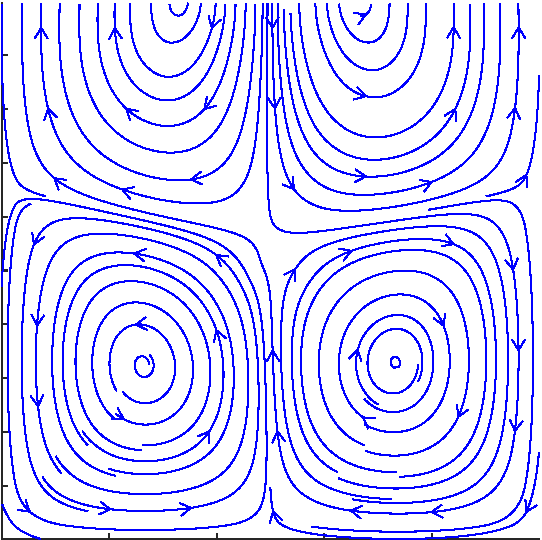
\includegraphics[width=0.72\textwidth]{figures/mean_uncontrolled_velocity_vort}};
%      \draw[line width=1pt] (0,0) rectangle (1,1) node[pos=0.5] {$D$};
%      \draw[line width=1pt, blue] (0,1) parabola bend (1/6,19/18) (1/3,1);
%      \draw[line width=1pt, blue] (1/3,1) parabola bend (1/2,8/9) (2/3,1) node[above, xshift=-0.4cm] {In/Outflow};
%      \draw[line width=1pt, blue] (2/3,1) parabola bend (5/6,19/18) (1,1);
%      \draw[line width=1.5pt, red] (0,0) -- (1,0) node[below left, xshift=-0.3cm] {Substrate};
%      \draw[line width=1.5pt, black!70!green] (0,0) -- (0,1) node[left, xshift=-0.3cm, yshift=-0.5cm, rotate=90] {Control};
%      \draw[line width=1.5pt, black!70!green] (1,0) -- (1,1) node[right, xshift=0.3cm, yshift=-0.5cm, rotate=-90] {Control};
%    \end{tikzpicture}
%\end{minipage}\hfill
%\begin{minipage}{0.65\textwidth}\vspace{-3mm}
%\[
%  \min_{z\in\Zad}\; \frac{1}{2}{\color{blue}\risk}\left[\int_{D} (\nabla\times V(z))
%    \,\mathrm{d}x\right] + \frac{\gamma}{2}\int_{\Gamma_c} |z|^2 \,\mathrm{d}x
%\]
%where $(V(z),P(z),T(z)) = (v,p,\tau)$ solves  \vspace{-1ex}
%\begin{align*}
%  -\alert{\nu(\omega)}\nabla^2 v + (v\cdot\nabla)v + \nabla p
%      + \alert{\eta(\omega)} \tau g &= 0
%    && \text{in }D \\
% %\nabla \cdot v &= 0 &&\text{in }D\\
%  -\alert{\kappa(\omega)} \Delta \tau + v\cdot\nabla \tau &= 0
%    && \text{in }D\\
%  \alert{\kappa(\omega)} \nabla \tau\cdot n + \alert{h(\omega)}(z-\tau) &=0
%    && \text{on }\Gamma_c
%\end{align*}
%\end{minipage}
%\begin{itemize}
%\item Find an equilibrium boundary temperature $z : \Gamma_c \to \mathbb R$ that minimizes the vorticity in CVD reactor.
%\item $V$ velocity, $P$ pressure, $T$ temperature.
%\item Possible random inputs:  kinematic viscosity $\alert{\nu}$, thermal expansion coefficient  $\alert{\eta}$, thermal conductivity $\alert{\kappa}$,  heat transfer coefficient due to rugosity $\alert{h}$. 
%\end{itemize}
%\end{block}
%\end{frame}

\section{State Constraints}

\begin{frame}\frametitle{Example: Constraints on the Random Field State Variable $u_{\xibold}$ }

\begin{block}{}
%\begin{itemize}
%\item 
Consider the \textbf{state constrained} problem:
\begin{subequations}
  \begin{align*}%\label{eq:optctrl}
  &\min_{z\in \mathcal{Z}_{\rm ad}} \; \frac{\kappa_s}{2}\mathbb{E}\left[\int_D ([u_{\xibold(\cdot)}(z)](x)-w(x))^2\,\mathrm{d}x\right]
                            + \frac{\kappa_c}{2}\| z \|^2_{L^2} \,\mathrm{d}x \\
  &\mathrm{subject\;to}\quad {\color{red}u_{\xibold(\cdot)}(z) \ge \psi \quad\text{a.e./a.s.},}
  \end{align*}
  where $u=u_{\xibold(\omega)}(z)\in H^1(D)$ is a weak solution to
%  \begin{align*}%\label{eq:pde}
%     -\nabla\cdot (\kappa(x,\xi)\nabla u(x)) + v(x,\xi)\cdot\nabla u(x) &= f(x,\xi) + z(x) &&\text{for $x\in D$} \\
%     \kappa(x,\xi)\nabla u(x)\cdot n &= 0 && \text{for $x\in\partial D \setminus [\{0\}\times(0,1)]$} \\
%     u(x) &= 0 && \text{for $x\in\{0\}\times(0,1)$}
%  \end{align*}
  \begin{align*}
  -\nabla\cdot({\epsilon(\xibold(\omega))}\nabla u) + {\mathbb{V}(\xibold(\omega))}\cdot\nabla u
    &= {f(\xibold(\omega))} - Bz &\quad\text{in $D$, a.s.}\\
  u &=0 &\quad \text{on $\Gamma_d = \{0\}\times(0,1)$, a.s.} \\
 { \epsilon(\xibold(\omega))}\nabla u\cdot n &= 0 &\quad\text{on $\partial D\setminus\Gamma_d$, a.s.}
\end{align*}
%  for realizations $\xibold = \xi$.
\end{subequations}

\end{block}
\centering{
 Motivation is the same as the deterministic case, but much more challenging.\\ \pause
 The state constraint can also be written as 
 \[
 \only<2>{
 \mathbb P(\left\{\omega \in \Omega \left| [u_{\xibold(\omega)}(z)](x) \ge \psi(x,\omega) \text{ a.e. } x \in D \right.\right\}) = 1}
%  \only<2>{
% \mathbb P(\left\{\omega \in \Omega \left| [u_{\xibold(\omega)}(z)](x) \ge \psi(x,\omega) \text{ a.e. } x \in D \right.\right\}) = 1}
% 
\]
 }
\end{frame}

\begin{frame}\frametitle{Some Recent Work (non exhaustive)}
\begin{thebibliography}{10}\tiny

\bibitem{MHFarshbaf_Shaker_RHenrion_DHoemberg_2018}
{\sc M.~H. Farshbaf-Shaker, R.~Henrion, and D.~H\"{o}mberg.}
\newblock Properties of chance constraints in infinite dimensions with an
  application to {PDE} constrained optimization.
\newblock  Set-Valued Var. Anal., 26(4):821--841, 2018.
\vspace{-1ex}

\bibitem{CGeiersbach_MHintermueller_2022}
{\sc C.~Geiersbach and M. Hinterm\"uller}
\newblock Optimality conditions and Moreau-Yosida regularization for almost sure state constraints.
\newblock  ESAIM: Control, Optimisation and Calculus of Variations (ESAIM: COCV): 28 (2022) 80
\vspace{-1ex}

\bibitem{CGeiersbach_WWollner_2021}
{\sc C.~Geiersbach and W.~Wollner}
\newblock Optimality conditions for convex stochastic optimization problems in Banach spaces with almost sure state constraints..
\newblock  SIAM Journal on Optimization 31(4): 2455-2480 (2021)
\vspace{-1ex}

\bibitem{DBGahururu_MHintermueller_TMSurowiec_2022}
{\sc D.B.~Gahururu, M.~Hinterm\"uller, and T.M.~Surowiec}
\newblock Risk-neutral PDE-constrained generalized Nash equilibrium problems. 
\newblock Math. Program. (2022). \url{https://doi.org/10.1007/s10107-022-01800-z}

\bibitem{DPKouri_MStaudigl_TMSurowiec_2022}
{\sc D.P.~Kouri, M.~Staudigl, and T.M.~Surowiec}
\newblock A Relaxation-based Probabilistic Approach for PDE-constrained Optimization under Uncertainty with Pointwise  State Constraints
\newblock Comput Optim Appl (2023). \url{https://doi.org/10.1007/s10589-023-00461-8}
\end{thebibliography}
\begin{block}{}

\begin{itemize} {\tiny
\item Farshbaf-Shaker et al. consider \textbf{probability constraints}
\item Geiersbach, Hinterm\"uller; Geiersbach, Wollner; Gahururu et al. consider \textbf{almost sure} formulation $+$ \textbf{constraint qualifications}.\vspace{-1ex}
\item Today's talk: Experience with the quadratic penalty approach and a new functional relaxation-based approach.
}
\end{itemize}
\end{block}
\end{frame}

\begin{frame}\frametitle{A Model Optimization Problem}
\begin{block}{}
\begin{itemize}
\item We consider a convex model problem for the analysis. Many results easily generalized. \pause
\item \textbf{Objective} 
\begin{equation}\label{eq:problem}
  j(z)\eqdef\Ex_{\Pr}[J(z,\xibold)],
\end{equation}
where $J(z,\xibold)$ convex in variables $z$ almost surely (a.s.)
and $\xibold$ denotes random inputs. \pause
\item \textbf{Bound constraints}\vspace{-2ex}
\begin{equation}\label{eq:Zad}
\setZ_{\rm ad} \eqdef \{v\in\scrZ\; \vert  \;a \le v \le b \text{ a.e.}\}.\vspace{-2ex}
\end{equation}\pause
\item \textbf{PDE-constraint}
For
fixed $z\in\scrZ$ and $\xi\in\Xi$, find $u_\xi \in H^1_0(D)$ that satisfies
\begin{equation}\label{eq:rpde_omega}
\begin{aligned}
 \int_{D} &\kappa(x,\xi)\nabla u_\xi(x) \cdot \nabla \phi(x) \dif x =  \int_{D} ((B(\xi)z)(x) + f(x,\xi))  \phi(x)  \dif x
 \quad\forall\,\phi\in H^1_0(D).
\end{aligned}
\end{equation} 
\item \textbf{Solution operator} 
$S_{\xi}:\scrZ\to H^{1}_{0}(D)$ solves  \eqref{eq:rpde_omega}, splits into $S_{\xi}(z)+u_{f(\cdot,\xi)}$ for $\xi\in\Xi$.\pause
\item \textbf{State constraints} 
\begin{equation}\label{eq:C}
\setC\eqdef\left\{z\in \setZ\, \vert\, \Pr\left(S_{\xibold}(z)[x]\geq\psi(x,\xibold)-u_{f(\cdot,\xibold)}(x)\quad\text{for a.a.\ }x\in D\right)=1\right\}.
\end{equation}

\end{itemize}
\end{block}
\end{frame}

\begin{frame}\frametitle{Technical Assumptions}
%\begin{block}{}
\begin{equation}\label{P}\tag{P}
  \inf_{z\in\setZ}\left\{ j(z) \,\vert\,  z\in\setC\cap\setZ_{\rm ad} \right\}
\end{equation}
%\end{block}
\begin{assumptions}[Structure of uncertainty]\label{as:pde}
\pause
\begin{enumerate}
\item 
\textbf{Bounded random forcing term} $f(\cdot,\xibold)\in L^{\infty}(\Omega,\scrF,\Pr; \scrZ)$;\pause
\item 
\textbf{Bounded random coefficients} There exist positive constants $0 < \kappa_0 \le \kappa_1 < +\infty$:
\[
  \kappa_{0}\le \kappa(\cdot,\xi)\le\kappa_{1} \quad \text{a.e.}\quad\forall\,\xi\in\Xi;
\]
\item \pause
\textbf{Sufficient compactness of control operator} Operator
$B(\xibold(\cdot)):\Omega\to\lin(\scrZ,H^{-1}(D))$ is measurable, bounded, and completely continuous:
\[
  z_{n} \wlim z\text{ in }\scrZ \quad\implies\quad B(\xibold)z_{n}\to B(\xibold)z \text{ in }H^{-1}(D)\quad\text{a.s.}
\]
\end{enumerate}
\end{assumptions}
\end{frame}

\begin{frame}\frametitle{Technical Assumptions}
%\begin{block}{}
%\begin{equation}\label{P1}\tag{P}
%  \inf_{z\in\setZ}\left\{ j(z) \,\vert\,  z\in\setC\cap\setZ_{\rm ad} \right\}
%\end{equation}
%\end{block}
\begin{assumption}[Domain, bound constraints, objective]\label{as:object_bounds}
\pause
\begin{enumerate}
\item \textbf{Deterministic domain} $D\subset\mathbb R^n$ open, bounded set with Lipschitz boundary
      $\Gamma\subset \mathbb R^{n-1}$;
\item \textbf{Control bounds} $a,b \in L^{2}(D)$ with $a<b$ a.e.;
\item \textbf{State bound} $\psi \in C({D}\times\Xi)$, $\psi(x,\xi)\leq 0$ on
      $\Gamma\times\Xi$, $\psi(\cdot,\xi) \in H^1(D)$
      for all $\xi\in\Xi$;
\item \textbf{Objective} $j(\cdot)$ is proper, weakly lower-semicontinuous, and convex.
\end{enumerate}
\end{assumption}\pause
\begin{assumption}[Existence of a feasible point]\label{ass:feas}
  The feasible set is nonempty, i.e., $\setC \cap \setZ_{\rm ad} \neq\emptyset$.
\end{assumption}
\pause

\centering{ 
Both algorithms can still be applied if feasibility is violated. 
}
\end{frame}

\section{Moreau-Yosida Regularization}
\begin{frame}[noframenumbering]\thispagestyle{empty}
\vspace*{\fill}
\begin{center}
\Large 
How can we treat the state constraints $\setC$ numerically?\\
\pause
Attempt \# 1: Quadratic penalty function
\end{center}
\vspace*{\fill}
\end{frame}

\begin{frame}\frametitle{Moreau-Yosida Regularization: Definition}
\begin{center}
The use of quadratic penalty functions to treat inequalities is often referred to as 
Moreau-Yosida regularization.
\end{center}
\begin{block}{}
Set
\[
\theta(z,\xi)\eqdef \psi(\cdot,\xi)-(u_{f(\cdot,\xi)}+S_{\xi}(z))
\]
and assume for illustration that
\[
j(z) := \frac{1}{2} \mathbb E_{\mathbb P}[\| S(z) + u_f - u_{d} \|^2_{L^2(D)}] + \frac{\nu}{2} \| z \|^2_{L^2(D)} \quad (\nu > 0).
\]
We consider a sequence of relaxed problems taking the form:
\begin{equation}\label{P-gamma}\tag{P$_\gamma$}
  \inf_{z\in\setZ}\left\{ j(z) + \frac{\gamma}{2} \mathbb E_{\mathbb P}[\| (-\theta(z,\xi))_+\|^2_{L^2(D)}] \,\vert\,  z\in\setZ_{\rm ad} \right\}.
\end{equation}
The functional
\[
 \mathbb E_{\mathbb P}[\| (-\theta(z,\xi))_+\|^2_{L^2(D)}] 
\]
can be seen as a measure of regret for violating (globally) the constraint.
\end{block}
\end{frame}

\begin{frame}\frametitle{Moreau-Yosida Regularization: Basic Theory}
\begin{block}{Asymptotic Behavior}
\begin{itemize}
\item Under a Slater-type constraint qualification and increased regularity assumptions, a limiting first-order optimality system can be derived along a subsequence of $\gamma \to +\infty$.
\item This guarantees asymptotic feasibility, the existence of Lagrange multipliers, etc.
\end{itemize}\pause
An interesting feature: 
\begin{itemize}
\item For finite $\gamma > 0$, the optimal solution satisfies $z_{\gamma} = \mathrm{Proj}_{\setZ_{\rm ad}}(-\mathbb E_{\mathbb P}[B^* \lambda_{\gamma}])$, where $\lambda_{\gamma}$
solves a ``typical'' adjoint equation.
\item For $\gamma \to +\infty$, the Bochner spaces for the random fields do not give sufficient compactness for $\lambda_{\gamma}$ to converge to a limiting adjoint state.
\item Instead, we are left with a kind of ergodic limit of $\Lambda$ as the weak limit of $\mathbb E_{\mathbb P}[B^* \lambda_{\gamma}]$.
\end{itemize}\pause
Even in this forgiving setting, the analysis is complex. See details (Thm. 4.4) in 

\begin{thebibliography}{10}\tiny
\bibitem{DBGahururu_MHintermueller_TMSurowiec_2022}
{\sc D.B.~Gahururu, M.~Hinterm\"uller, and T.M.~Surowiec}
\newblock Risk-neutral PDE-constrained generalized Nash equilibrium problems. 
\newblock Math. Program. (2022). \url{https://doi.org/10.1007/s10107-022-01800-z}
\end{thebibliography}
\end{block}
\end{frame}

\begin{frame}\frametitle{Moreau-Yosida Regularization: Relation to Probability Constraints}
\begin{theorem}[Gahururu, Hinterm\"uller, Surowiec (2022)]\label{prop:markov}
Let $z_{\gamma}$ be the (unique) minimizer of \eqref{P-gamma}. Then for any $\varepsilon > 0$, we have
 \begin{equation*}
  \mathbb P \left(  \| (-\theta(z_{\gamma},\xibold)_+ \|^2_{L^2(D)} < \varepsilon \right) \geq 1 - \frac{2M}{\gamma \varepsilon},
 \end{equation*}
where $M = \mathbb{E}_{\mathbb P}\left[ J(S(z),z)\right] $ and $z$ is the unique minimizer of \eqref{P}.
\end{theorem}
\begin{itemize}
\item Proof: Use Markov's inequality, feasibility of $z^{\gamma}$, definition of optimality.\pause
\item Implication: Using the convergence theory for $\gamma \to +\infty$, properties of convergence in distribution, Slutsky's theorem, the Portmanteau lemma, and $\varepsilon = 1/\sqrt{\gamma}$ gives:
\[
 1 = \limsup_{\gamma} 1 - \frac{2M}{\sqrt{\gamma}} \le \pause \limsup_{\gamma} \mathbb P \left(  \| (-\theta(z_{\gamma},\xibold)_+ \|^2_{L^2(D)} \le 1/\sqrt{\gamma} \right)\pause \le  \mathbb P \left(  \| (-\theta(z,\xibold)_+ \|^2_{L^2(D)} \le 0\right) = 1
\]\pause
\end{itemize}
\centering{
We thus obtain a ``probabilistic'' rate of convergence to feasibility like. e.g., $1 - 2M/\sqrt{\gamma}$.

}
\end{frame}

\begin{frame}\frametitle{Empirical Approximation, Semismooth Newton, and Path-Following}
\begin{block}{}
\begin{itemize}
\item When solving OUU problems, we typically need to approximate $\mathbb P$.
\item Given a sample of size $N$, we can consider the empirical probability measure $\mathbb P_N$.
\item This is sometimes referred to as ``Sample Average Approximation'' (SAA)\footnote{\tiny See the survey A. Shapiro \textit{Monte Carlo sampling methods} In A. Ruszczynski and A. Shapiro, editors, Stochastic
Programming, Handbooks in Operations Research and Management Science. Elsevier, 2003.}.\pause
\item In essence, we consider \alert{deterministic}, \alert{sample-based} problems of the type
\begin{multline}\label{SAA}\tag{P$_{\gamma}(\mathbb P_N)$}
  \min_{z \in Z_{\rm ad}}
\left\{ 
\frac{1}{N} \sum_{i=1}^N\left[ J(z,\xibold^i(\omega^i)) +\frac{\gamma}{2} \| (-\theta(z_{\gamma},\xibold^i(\omega^i)))_+ \|^2_{L^2(D)}\right]
\right\}
\end{multline}
\item \pause Solutions $z^N_{\gamma}$ are \alert{random} due to the dependence on $\mathbb P_N$, which itself based on the r.s. $(\xibold^1,\dots,\xibold^N)$. 
\item \pause Since \eqref{SAA} is a deterministic PDE-constrained problem, we can use existing solvers.
\item  \pause The hidden cost: \alert{not one PDE-constraint but N}! Meaning potentially \alert{thousands of PDE-constraints}.
\end{itemize}
\end{block}
\end{frame}

\begin{frame}\frametitle{Empirical Approximation, Semismooth Newton, and Path-Following}
\vspace{-2ex}
\begin{block}{}
\begin{itemize}
\item The favorable structure allows the application of a \alert{semismooth Newton method}.
\item This needs to be coupled with a \alert{continuation strategy/path-following} for $\gamma$.\pause
\item For each $i=1,\dots, N$, there is a forward equation yielding a state $u_{\gamma}^i$ and adjoint equation for $\lambda_{\gamma}^i$.
\item The solutions to \eqref{SAA} have the form:
\begin{equation*}%\label{eq:first_order_M}
z^{N}_{\gamma} = \mathrm{Proj}_{Z_{ad}}\left[-\frac{1}{\nu N} \sum_{i=1}^N B^*(\xi^i(\omega^i)) \lambda^{i}_{\gamma} \right],
\end{equation*}
\item \pause The adjoint equations take the form
  \[
  \int_{D} \kappa(x,\xi^i)\nabla \lambda(x) \cdot \nabla v(x) \dif x  = \int_{D}(u_{\gamma}^i - u_d + \mu_{\gamma}^i) v(x)  \dif x
    \quad\forall\,v\in H_0^1(D),
    \]
    where 
$
\mu_\gamma^{i} = -\gamma  (\psi^i - ({u}_{\gamma}^i + u_f^i))_+.
$
\item \pause We define the mapping $z \mapsto B^* \lambda^{\gamma}$ as $\Lambda(z)$ or $\Lambda(z,\omega)$ to indicate the dependence on $\omega$. 
\item This mapping is \alert{nonsmooth}.
\end{itemize}
\end{block}
\end{frame}

\begin{frame}\frametitle{Empirical Approximation, Semismooth Newton, and Path-Following}
\begin{block}{}
\begin{itemize}
\item The \alert{nonsmooth} residual used for our algorithm is 
 \[
F_{\gamma}^{N}(z) := z - \mathrm{Proj}_{Z_{ad}}\left[-\frac{1}{\nu N} \sum_{i=1}^N \Lambda(z,\omega^i)\right] = 0.
\]
\item \pause $F_{\gamma}^{N} : L^2(D) \to L^2(D)$ admits a \alert{Newton derivative} $G_{\gamma}^{N}(z)$ of the form
\[
G_{\gamma}^{N}(z) dz =
\left[I + \frac{1}{\nu N} \sum_{i=1}^N \mathcal{G}\left[\Lambda(z,\omega^i)\right] \Lambda'(z,\omega^{i})\right] dz,
\]
where $\mathcal{G}$ and $\Lambda'(z,\omega^i)$ are the \alert{Newton derivatives of the projection operator and adjoint}, resp. 
\item \pause This allows us to apply a semismooth Newton method in $L^2(D)$\footnote{\tiny
See e.g., M. Hintermüller, K. Ito, and K. Kunisch \textit{The primal-dual active set strategy as a semismooth Newton method} SIAM J. Optim., 13(3):865–888 (2003)
and
M. Ulbrich \textit{Semismooth Newton methods for operator equations in function spaces} SIAM J. Optim., 13(3):805–842 (2003).}, 
which is locally superlinearly convergent for each $N$ and $\gamma > 0$. 
\item $G^N_{\gamma}(z)$ \alert{cannot be} computed explicitly, need iterative method for \alert{generalized Hessian vector products}.
\end{itemize}
\end{block}
\end{frame}

\begin{frame}\frametitle{Comments}
%The basic idea behind this algorithm derives from the success of semismooth Newton methods for solving deterministic PDE-constrained optimization problems subject to state constraints using Moreau-Yosida regularization and path-following for the parameter updates; see e.g., \cite{MHintermueller_KKunisch_2006A,MHintermueller_KKunisch_2006B}.
%Indeed, given $\gamma > 0$ and an iid sample of size $M$, we can replace the underlying probability distribution with the associated empirical probability measure $\mathbb P_M$ and consider 
%\begin{multline}\label{eq:single_player_opt_MY_M}
%% \min_{z \in Z_{\rm ad}}
%%\left\{ 
%%\mathbb E_{\mathbb P_{M}}\left[J(S(z)+ u_f,z) +\frac{\gamma}{2} \| (\psi - (S(z) + u_f))_+ \|^2_{L^2(D)}\right] 
%%\right\} =\\
%  \min_{z \in Z_{\rm ad}}
%\left\{ 
%\frac{1}{M} \sum_{m=1}^M \left[J(S(z)(\omega^m)+ u_f(\omega^m),z) +\frac{\gamma}{2} \| (\psi(\omega^m) - (S(z)(\omega^m) + u_f(\omega^m)))_+ \|^2_{L^2(D)}\right] 
%\right\}.
%\end{multline}
%This is now a deterministic problem. In order to solve \eqref{eq:single_player_opt_MY_M} with a semismooth Newton solver, we rewrite the first order optimality system as a single nonsmooth equation in $z$.
%\begin{equation}\label{eq:first_order_M}
%z^{\gamma, M} = \mathrm{Proj}_{Z_{ad}}\left[-\frac{1}{\nu M} \sum_{m=1}^M B^*(\omega^m) \lambda^{\gamma}_{m} \right],
%\end{equation}
%where for each $m =1,\dots, M$, $\lambda^{\gamma}_m \in H^1_0(D)$ solves
%\begin{equation}\label{eq:apde_omega_gamma_m}
% \int_{D} A(x,\omega^{m})\nabla {\lambda}^\gamma_m (x) \cdot \nabla \varphi(x) \ \mathrm{d} x   =  \int_{D} ( T^*( T{u}^{\gamma}_m + Tu_f(\omega^{m}) - u_d)+{\mu}^{\gamma}_m))  \varphi(x)  \ \mathrm{d} x,
%\end{equation}
% for all $\varphi \in H^1_0(D)$, ${u}^{\gamma}_m = S({z}^{\gamma,M})(\omega^{m}) \in H^1_0(D)$ solves
%\begin{equation}\label{eq:rpde_omega_m}
% \int_{D} A(x,\omega^{m})\nabla {u}^{\gamma}_m (x) \cdot \nabla \varphi(x) \ \mathrm{d} x   =  \int_{D} (B(\omega^{m}){z}^{\gamma,M})(x)  \varphi(x)  \ \mathrm{d} x,
%\end{equation}
%\begin{equation}\label{eq:rpde_omega_m}
% \int_{D} A(x,\omega^{m})\nabla {u}^{\gamma}_m (x) \cdot \nabla \varphi(x) \ \mathrm{d} x   =  \int_{D} ((B(\omega^{m}){z}^{\gamma,M})(x)+ f(x,\omega^{m}))  \varphi(x)  \ \mathrm{d} x,
%\end{equation}
%with the same test functions $\varphi$, and 
%\[
%\mu^\gamma_{m} = -\gamma  (\psi(\omega^m) - ({u}^{\gamma}_m + u_f(\omega^m)))_+.
%\]
%The fixed random terms $u_{f}(\omega^{m})$ are defined analogously to $u^{\gamma}_m$.
%For readability, we denote the mapping $z \mapsto B^* \lambda^{\gamma}$ as $\Lambda(z)$ or $\Lambda(z,\omega)$ to indicate the dependence on $\omega$. Moreover, we set
%\[
%F^{\gamma}_{M}(z) := z - \mathrm{Proj}_{Z_{ad}}\left[-\frac{1}{\nu M} \sum_{m=1}^M \Lambda(z,\omega^m)\right].
%\]
%In the current setting, $F^{\gamma}_{M} : L^2(D) \to L^2(D)$ admits a Newton derivative $G^{\gamma}_{M}(z)$ of the form
%\[
%G^{\gamma}_{M}(z) dz =
%\left[I + \frac{1}{\nu M} \sum_{i=1}^M \mathcal{G}\left[\Lambda(z,\omega^m)\right] \Lambda'(z,\omega^{m})\right] dz,
%\]
%where $\mathcal{G}$ is the Newton derivative of the projection operator. This allows us to apply a semismooth Newton method in $L^2(D)$ \cite{MHintermueller_KIto_KKunisch_2002,MUlbrich_2002}, which is known to be locally superlinearly convergent for each $M$ and $\gamma > 0$. 

\begin{block}{}
\begin{itemize}
\item $N$ determines the accuracy of the approximation of the expectations.
\item We use Monte Carlo, i.e. the accuracy is on the order of $O(N^{-1/2})$.
\item $\gamma$ must be taken to $+\infty$, so large $N$ for small $\gamma$ does not make sense.
\item Heuristic: set a maximum allowable sample size $N_{\rm max} > 0$ and penalty parameter $\gamma_{\rm max} > 0$. Start with small $N_0 \in \mathbb N$ and $\gamma_0 > 0$, and add samples to $N_k$ every time $\gamma_k$ passes a certain threshold.
\item Gahururu, Hinterm\"uller, Surowiec (2022) provides some mathematical justification.
\item All Newton steps for each $\gamma_k$ are inexact with tolerance ${\tt tol^{newt}} \ge 0$.
\item We use CG for the iterative solver.
\end{itemize}
\end{block}

%However, since $\gamma$ must be taken to $+\infty$, such an algorithm would not be computationally efficient if $M$ were chosen large for comparatively small $\gamma$.  If $M$ were to remain fixed, then we could use a strategy as in \cite{MHintermueller_KKunisch_2006A,MHintermueller_KKunisch_2006B,LAdam_MHintermueller_TMSurowiec_2019}. On the other hand, $M$ should be ideally as large as possible or also treated as a parameter going to $+\infty$. To remedy this issue, we set a maximum allowable sample size $M_{\rm max} > 0$ and penalty parameter $\gamma_{\rm max} > 0$ and, starting with $M_0 \in \mathbb N$ and $\gamma_0 > 0$, we add samples to $M_k$ every time $\gamma_k$ passes a certain threshold. For our numerical experiments, we consider a heuristic, which is motivated by the previous section; in particular the convergence statements in the fully continuous setting along with Remarks \ref{rem:ergodic_adjoint} and \ref{rem:prob_rate}. A full convergence analysis linking sampling, approximation and smoothing error goes beyond the scope of this paper. The full algorithm is given in Algorithm \ref{alg:SA}. A few comments are in order.

%The operator $G^{\gamma_k}_{M_k}(z^k_{l})$ is not explicitly given. Thus, it is necessary to use an iterative method to solve for the Newton steps $dz^{k}_{l}$, for which we use the tolerance ${\tt tol^{newt}} \ge 0$. Since we are using a semismooth Newton iteration for pointwise bound constraints, the components of $dz^{k}_{l}$ are fixed on the estimated active sets for each $l$ and we only need to solve the linear systems on the potentially smaller inactive set.  Here, it is important to note that each evaluation of $G^{\gamma_k}_{M_k}(z^k_l) dz^k_l$ requires the solution of the forward equation and two adjoint equations for every sample $m_k = 1,\dots,M_k$. In our implementation, we employ a preconditioned conjugate gradient method. Therefore, the computational complexity of each Hessian-vector product involved must also be multiplied by $M_k$ and take into account the cost of applying the preconditioner.  Similarly, the evaluation of the residual $F^{\gamma}_{M_k}(z^{k}_{l})$ requires a forward and adjoint solve for each sample.  For our numerical examples, we use a direct solver for the linear elliptic PDEs.

%Due to these facts, we suggest starting with a relatively small $M_0$ and increasing slowly with $\gamma_k$. Moreover, we suggest a relatively large ${\tt tol}^{\rm res}_{0} > 0$ and $\rho^{\rm res}$ close to 1. In step 13: of Algorithm \ref{alg:SA}, we simply set $\gamma_{k+1} = \phi(\gamma_k) = \gamma_k + 1$. More aggressive strategies may be possible, but empirical evidence suggests that this is not necessary and may even cause the Newton iteration to cycle. Finally, in step 15: of Algorithm \ref{alg:SA},  we link the increases of the sample sizes $M_k$ to $\gamma_k$. For our implementation, we start with $\gamma_0$ and $M_0$ and increase $M_k$ by $10$ every time $\gamma_k$ is divisible by $100$. 
\end{frame}

\begin{frame}\frametitle{The Algorithm}\tiny
\begin{algorithm}[H]
 \caption{SSN for Stochastic PDE-Constrained Optimization with State Constraints}
 \label{alg:SA}
 {\LinesNotNumbered 
 \begin{algorithmic}
\STATE {\bf Input (Data):} $u_d \in L^2(D)$; $\nu > 0$; $a,b \in L^{\infty}(D)$ $a < b$; $\psi \in C(\overline{\Xi})$;  $f \in L^{\infty}_{\mathbb P}(\Omega; L^2(D))$
\STATE {\bf Input (Parameters):} $k : = 0$, 
$\gamma_0 > 0$,
$\gamma_{\rm max} \ge \gamma_0 > 0$,
$N_{0} \in \mathbb N$,  
$N_{\rm max} \ge M_{0}$, 
$\phi : \mathbb R_+ \to \mathbb R_+$,  
${\tt tol}^{\rm res}_0 > 0$, 
$\rho^{\rm res} \in (0,1)$, 
${\tt tol}^{\rm newt} \ge 0$
\STATE {\bf Input (Initial Values):}  $z_0 \in L^2(D)$, $dz_{0} \equiv 0 \in L^2(D)$
\WHILE{  $\gamma_k < \gamma_{\rm max}$ }
\STATE Set $l := 0$
\STATE Set $z^{k}_{l} := z_k$
\WHILE{ $\| F_{\gamma_k}^{N_k}(z^k_{l}) \| > {\tt tol}^{\rm res}_{k}$}
\STATE Find $dz^{k}_{l} \in L^2(D)$ such that 
\begin{equation*}%\label{eq:inner_newton_update}
\| G_{\gamma_k}^{N_k}(z^{k}_{l}) dz^{k}_{l} + F_{\gamma_k}^{N_k}(z^{k}_{l}) \|_{L^2(D)} \le {\tt tol^{\rm newt}}
\end{equation*}
\STATE  Set $z^{k}_{l + 1} := z^{k}_{l} + dz^{k}_{l}$
\STATE  Set $l := l + 1$
\ENDWHILE
\STATE Set $z_{k+1} = z^{k}_{l}$
\STATE Set $\gamma_{k+1} = \phi(\gamma_k)$
\IF{``penalty-to-sample threshold'}
\STATE Choose $N_{k+1} \in [N_{k},N_{\rm max}]$
\ELSE{}
\STATE Set $N_{k+1} := N_k$
\ENDIF
\STATE Set ${\tt tol}^{res}_{k+1} = \rho {\tt tol}^{res}_{k}$
\STATE Set $k := k + 1$
\ENDWHILE
\end{algorithmic}
}
\end{algorithm}
\end{frame}

\begin{frame}\frametitle{Performance Test in 1D}
\vspace{-1ex}
\begin{example}
Consider
\begin{equation*}%\label{eq:model_op}
  \operatorname*{minimize}_{z\in\setZ_{\rm ad}} 
     \frac{1}{2} \mathbb E_{\mathbb P}\left[ \| u- \widetilde{u}_{d} \|^2_{L^2(D)}\right]
    +\frac{\nu}{2} \| z \|^2_{L^2(D)}\text{ over } z \in L^2(D)
\end{equation*}
where $z \in 
\setZ_{\rm ad} := \left\{w \in L^2(D) \left| -0.75 \le w(x) \le 0.75\right.\right\}
$
 and 
 $u=u(z)\in L^{\infty}(\Omega, \mathcal{F}, \mathbb P;H^1(D))$ solves 
\begin{subequations} \label{eq:elliptic_equation}
\begin{align}
  -\alpha(\omega) \partial_{xx} u(\omega,x) &= f(\omega,x) + z(x) 
           \quad &(\omega,x)\in\Omega\times D, \\
     u(\omega,0) = d_0(\omega),\quad u(\omega,1) &= d_1(\omega) \quad &\omega\in\Omega. 
\end{align}
\end{subequations}
Here, we assume
\[
\aligned
\alpha(\omega) &:= 10^{2\xi_1(\omega)-3},\quad f(\omega,x) := \frac{2\xi_2(\omega)-1}{10},\quad
d_0(\omega) := 2+\frac{2\xi_3(\omega)-1}{1000}\quad
d_1(\omega) :=  1+ \frac{\xi_4(\omega)}{1000},
\endaligned
\]
with uniform r.v. $\xi_i :\Omega \to \mathbb R$, $i=1,2,3,4$, such that the supports $\xi_i$, $i=1,2,3,4$, are $[0,1]$. 
In addition, we impose the state constraint
\[
\mathbb P(\left\{\omega \in \Omega \left|\; u(\omega,x) \ge 0, \text{ for } \mathcal{L}\text{-a.e. } x \in D \right.\right\}) = 1.
\]
and
set $\nu = 10^{-3}$, 
$D = (0,1)$, $\widetilde{u}(x) = \sin(50.0*x/\pi)$
\end{example}
%In order to demonstrate the viability of the algorithm, we consider a model problem 
% based on \cite[Ex. 6.1, Ex. 6.2]{DPKouri_TMSurowiec_2016a} and \cite[Sec. 7.2]{MHoffhues_WRoemisch_TMSurowiec_2020}. Here, we set , and consider the optimal control problem


%Furthermore, we suppose that 
%\[
%\aligned
%\nu(\omega) &:= 10^{2\xi_1(\omega)-3},\quad
%&f(\omega,x) &:= \frac{2\xi_2(\omega)-1}{10}\\
%d_0(\omega) &:= 2+\frac{2\xi_3(\omega)-1}{1000}\quad
%&d_1(\omega) &:=  1+ \frac{\xi_4(\omega)}{1000},
%\endaligned
%\]
%with random variables $\xi_i :\Omega \to \mathbb R$, $i=1,2,3,4$, such that the supports $\xi_i$, $i=1,2,3,4$, are $[0,1]$. 
%We assume here that each of these random variables is uniformly distributed. Following the usual change of variables, the forward problem \eqref{eq:elliptic_equation} can be understood as 
%\begin{subequations} \label{eq:elliptic_equation_2}
%\begin{align}
%  -\nu(\xi) \partial_{xx} u(\xi,x) &= f(\xi,x) + z(x) 
%           \quad &(\xi,x)\in\Xi\times D, \\
%     u(\xi,0) = d_0(\xi),\quad u(\xi,1) &= d_1(\xi) \quad &\xi\in\Xi. \label{seq:elliptic_equation_b}
%\end{align}
%\end{subequations}
%with $\Xi = [0,1]^4$, endowed with the associated uniform density. We define $\bm \xi := (\xi_1,\dots,\xi_4) \in \Xi$. Since \eqref{eq:elliptic_equation_2} is linear, we can use the superposition principle to lift the boundary conditions into the righthand side of \eqref{eq:elliptic_equation_2}. This allows us to transform the problem into the function space setting used throughout the paper.
\end{frame}

\begin{frame}\frametitle{Performance Test in 1D: Parameters}
\begin{block}{}
\begin{itemize}
\item Control and state spaces discretizes using continuous Lagrange FE (P1): uniform grid, mesh parameter $h = 1/(2^{9}-1)$.
\item Random samples generated with standard Monte Carlo (sort of...)
\item Sample size $N_k$ linked to penalty parameter $\gamma_k$: 
\item  Set $\gamma_0 = 1$, $\gamma_{\rm max} = 10^4$, $M_0 = 200$, ${\tt tol}^{\rm res}_{0} = 10^{-2}$, $\rho^{\rm res} = 0.9997$, ${\tt tol}^{\rm newt} = 10^{-8}$
\item  Once the penalty to sample threshold is reached, $M_k$ is increased by 10 samples.
\item $z_0 \equiv 0$
\item PDE solved with LU, Newton iterates with PCG (using ``localized'' mass matrix for inactive set).
\item Nonlinear (nonsmooth) operator in adjoint equation treated with mass-lumping.
\end{itemize}
\end{block}
%\subsubsection{Discretization and Implementation}\label{ssec:pde_opt_dis} 
%The pointwise forward problem and the control space are discretized using piecewise finite elements on a uniform mesh with parameter $h = 1/(2^{9}-1)$. We use a standard Monte Carlo approximation for the random inputs $\xi_1,\dots,\xi_4 \in [0,1]$. We initialize the algorithm by choosing: $\gamma_0 = 1$, $\gamma_{\rm max} = 10^4$, $M_0 = 200$, ${\tt tol}^{\rm res}_{0} = 10^{-2}$, $\rho^{\rm res} = 0.9997$, ${\tt tol}^{\rm newt} = 10^{-8}$, $z_0 \equiv 0$. Once the penalty to sample threshold is reached, $M_k$ is increased by 10 samples. As mentioned above, the discrete PDEs are solved via a direct solver and the Newton steps are calculated using a preconditioned method of conjugate gradients (for the linear equation on the inactive set). As a preconditioner we use the localized mass matrix for the inactive set. 
%The stopping criterion for the inner loop works as follows. 
%The nodal values for the control and adjoint states are used in the pointwise projection formula for the bound constraints in $F^{\gamma_k}_{M_k}$. These values are interpolated in the nodal basis and the discrete $L^2(D)$ norm is calculated. 
%In the current implementation, we use the $\ell^2$-norm of the residual in the stopping criterion. Alternatively, one could use the proper discrete Riesz maps (i.e. the inverse mass matrix) to first obtain a representation of the discrete solution in the finite-dimensional subspace and then use the discrete $L^2$-norm. This would be especially important in a nested grid or AFEM approach in future numerical studies.
%For the nonsmooth operator in the adjoint equations, we utilize a mass-lumping approach to obtain the discrete operators. Otherwise, the differential operators and identity operators give rise to the usual stiffness and mass matrices subject to the random inputs.
\end{frame}

%\begin{frame}
%\subsubsection{Performance of the Algorithm}\label{ssec:pde_opt_perf}
%\begin{enumerate}
%\item Save total number of CG iterations
%\item Plot the number of CG iterations over $k$
%\item Save total number of Newton iterations per $\gamma_k, M_k$ pair
%\item Plot the number of Newton iterations over $k$
%\item Mention what doesn't seem to work: Small samples on the order to 10 fail with the current strategy.
%\item 
%\end{enumerate}

%The performance of the algorithm can be seen in Figure \ref{fig:pcg_nwt}, where we plot the total number of PCG iterations per $\gamma$-update ($k$) and the total number of Newton iterations needed to reach $\gamma = 1000$. The number of PCG iterations remains relatively stable (between 100-150), whereas the number of Newton iterations per $\gamma$-update appears to be trending downward. We note that no more than five Newton steps were needed for any given $\gamma$ and that both the CG algorithm and inner loop used inexact solves. Since we employed a relatively rough initial stopping tolerance and a small batch of samples (despite increasing by 10 everytime $(\gamma_k\,\mod 100) = 0$) the algorithm consistently produces a solution $\overline{z}$ that performs exactly as expected in light of the model (risk neutral objective) and theory (especially Remark \ref{rem:prob_rate}). This is qualitatively illustrated in Figure \ref{fig:z_oos}, where we observed that only 2.3 \% of  the out-of-sample states violated the bound constraint. 
%%Since we are using a risk-neutral objective function, the solution $\overline{z}$ is supposed to perform well on average. In order to illustrate this, we plot the average of 2000 out-of-sample states versus the desired state $u_d$. 
%Due to the presence of the random viscosity term in the forward problem, the $L^{\infty}$-norm of the sampled states can vary significantly.  Finally, and perhaps due to the previous fact, we noticed that smaller batches sizes, e.g., on the order of 10, led to a  failure of the Newton solver for $\gamma$ near 1000.

%\begin{figure}[!ht]
%  \centering
%  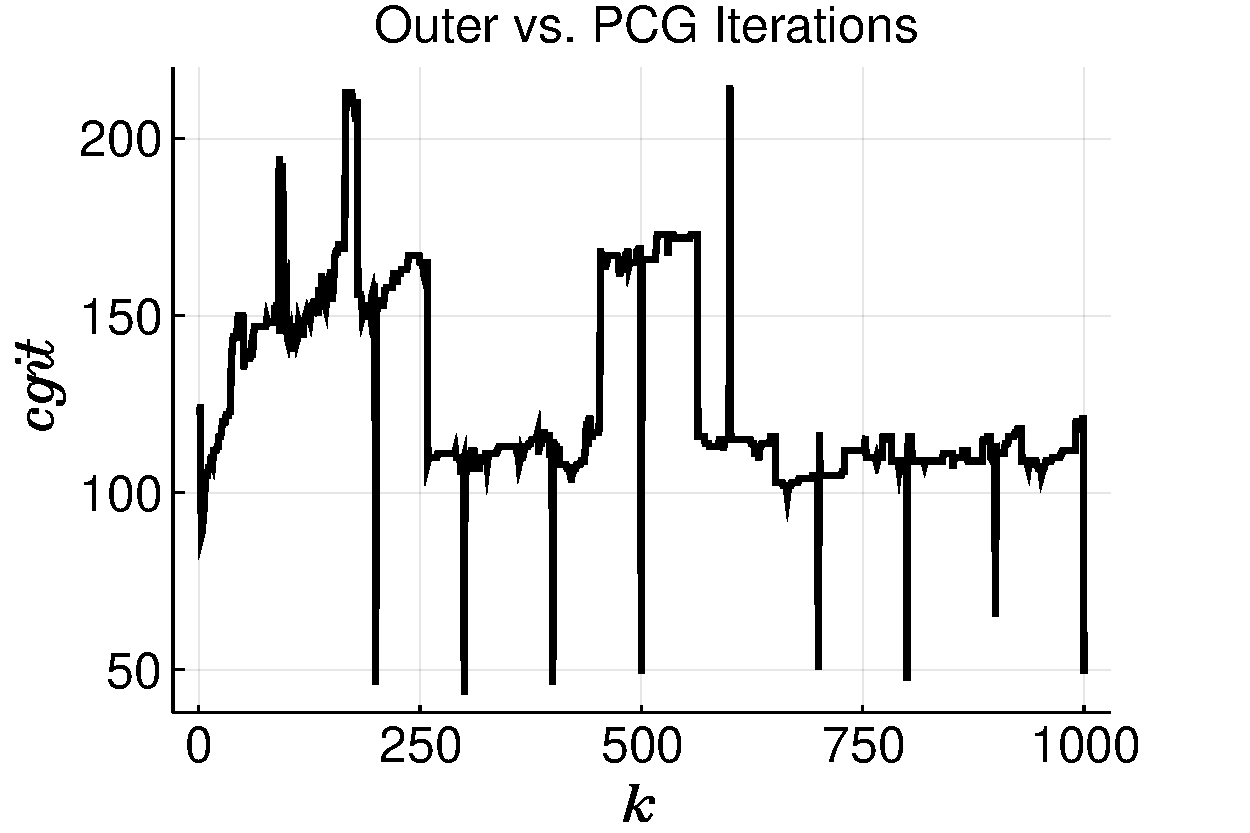
\includegraphics[width=0.47\textwidth]{figures/cg_vec_my_1000.pdf}
%  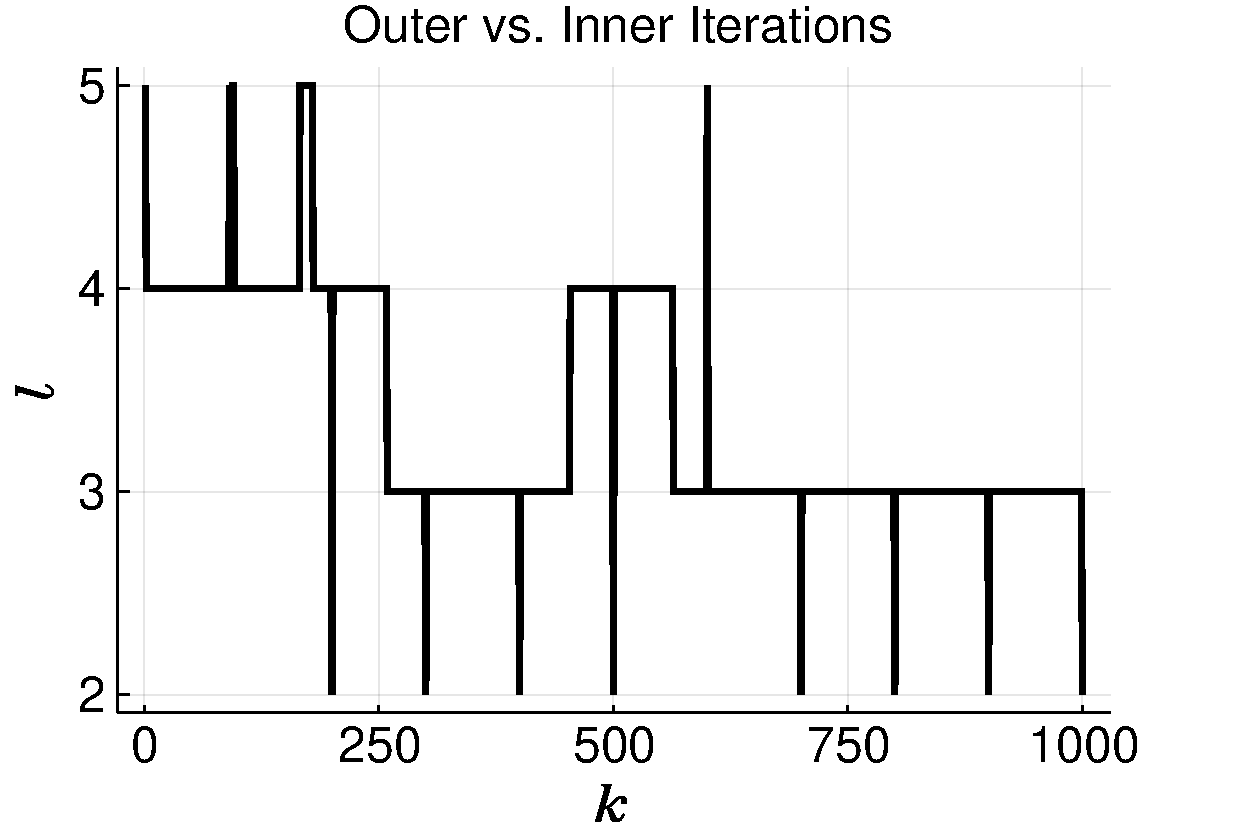
\includegraphics[width=0.45\textwidth]{figures/nwt_vec_my_1000.pdf}
%%  \caption{(left) Total PCG iterations per outer iteration k. (right) Total Newton iterations per outer iteration k.}
%%  \label{fig:pcg_nwt}
%\end{figure}
%
%\begin{figure}[!ht]
%  \centering
%  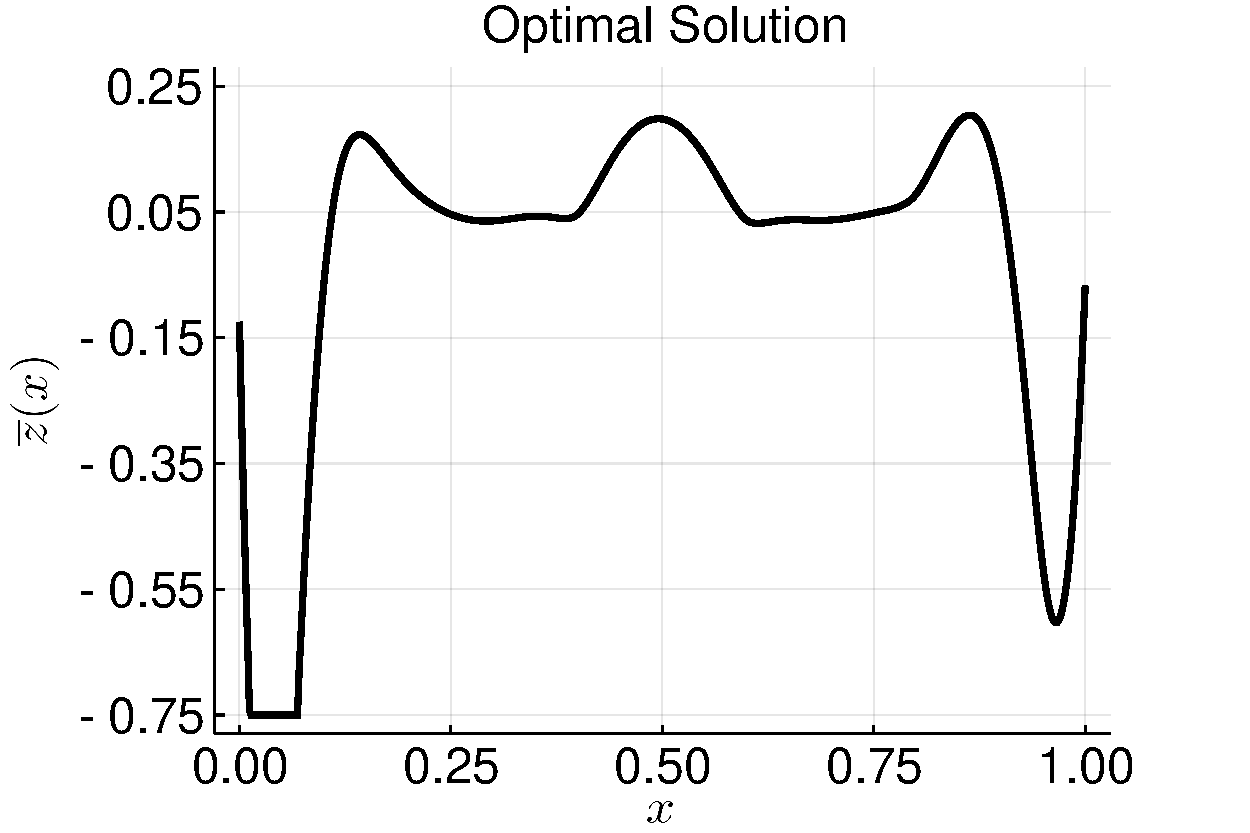
\includegraphics[width=0.45\textwidth]{figures/z_my_1000.pdf}
%  \includegraphics[width=0.45\textwidth]{figures/oos_my_g1000_M2000.pdf}
%%  \caption{(left) Optimal solution $\overline{z}$ up to $\gamma = 1000$. (right) Controlled states using $\overline{z}$ for 2000 out of sample instances of $\bm\xi$. }
%%  \label{fig:z_oos}
%\end{figure}
%\end{frame}

%\begin{frame}\frametitle{Results of Moreau-Yosida Penalty Approach}
%\begin{figure}[!ht]
%\begin{minipage}{0.49\textwidth}
%  \centering
%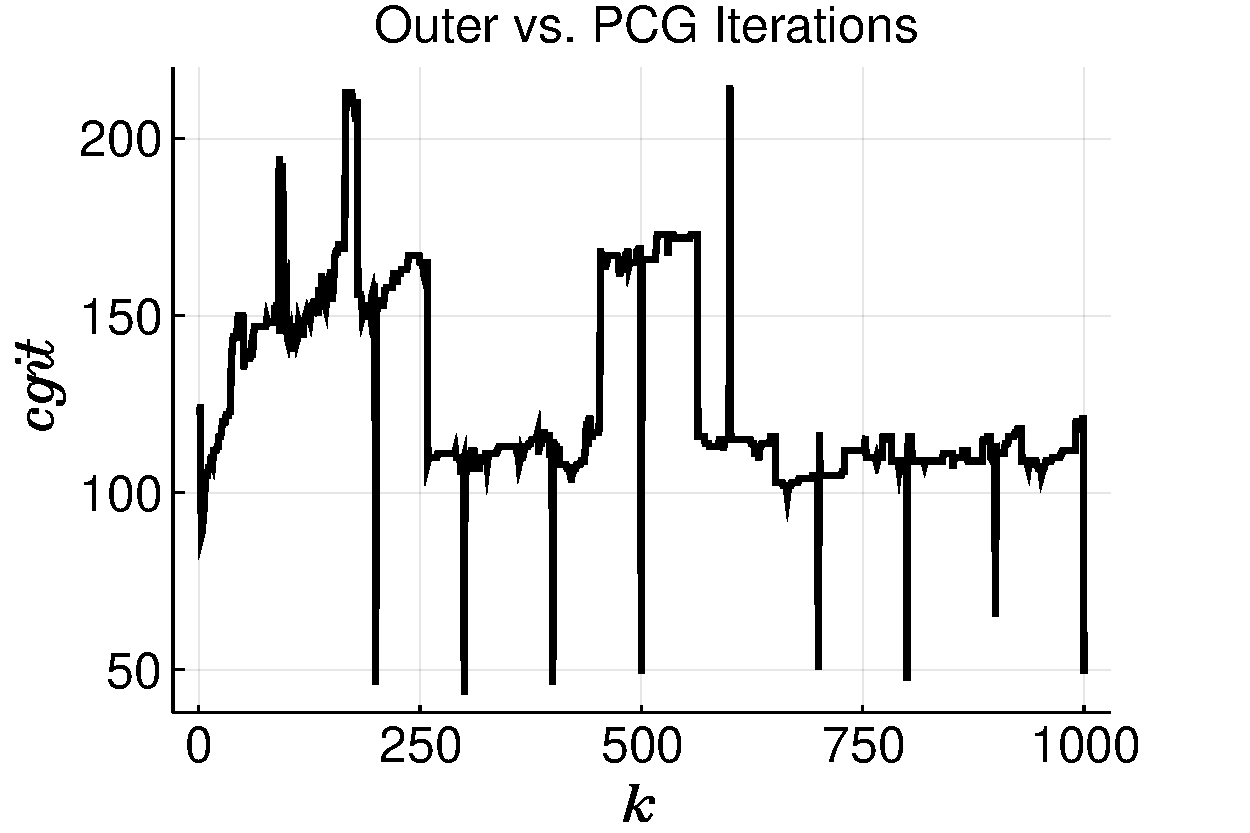
\includegraphics[width=0.47\textwidth]{figures/cg_vec_my_1000.pdf}
%  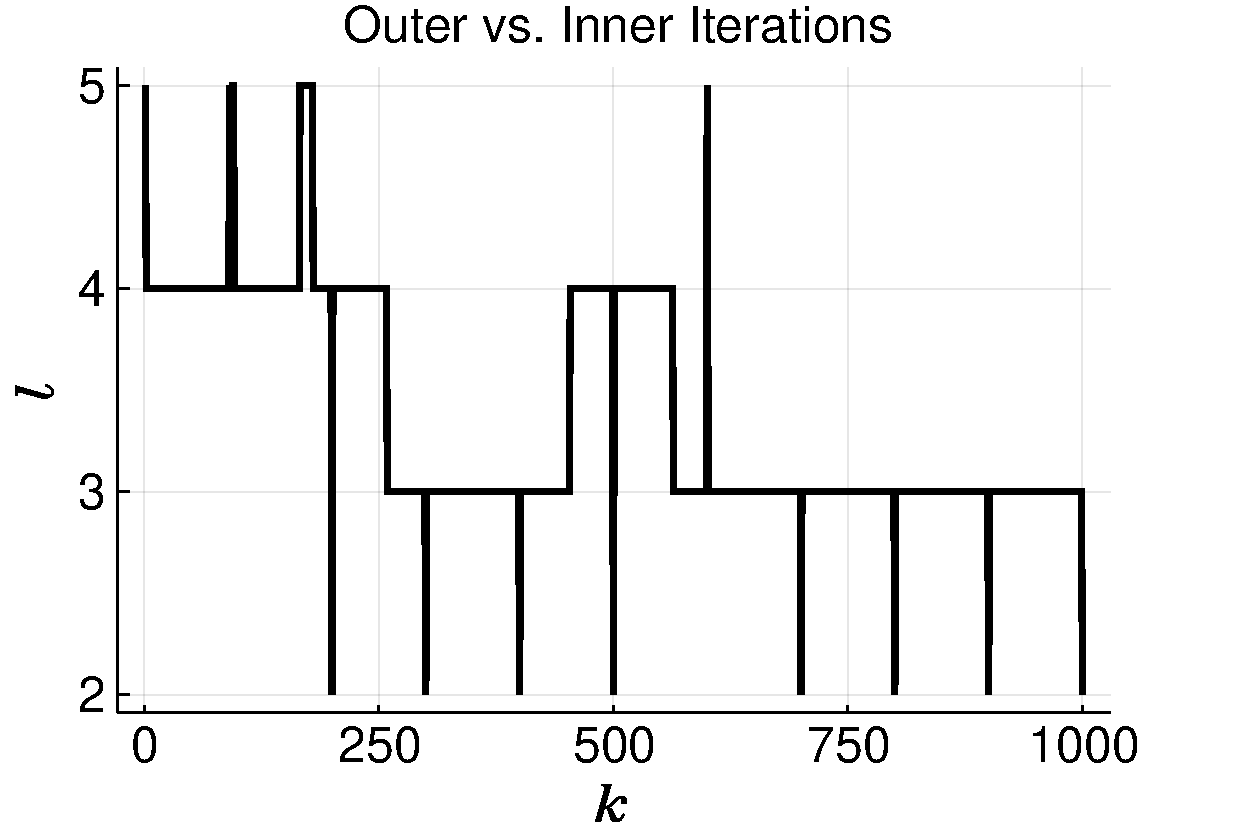
\includegraphics[width=0.47\textwidth]{figures/nwt_vec_my_1000.pdf}
%%  \caption{(left) Total PCG iterations per outer iteration k. (right) Total Newton iterations per outer iteration k.}
%\end{minipage}
%\begin{minipage}{0.49\textwidth}
%  \centering
%  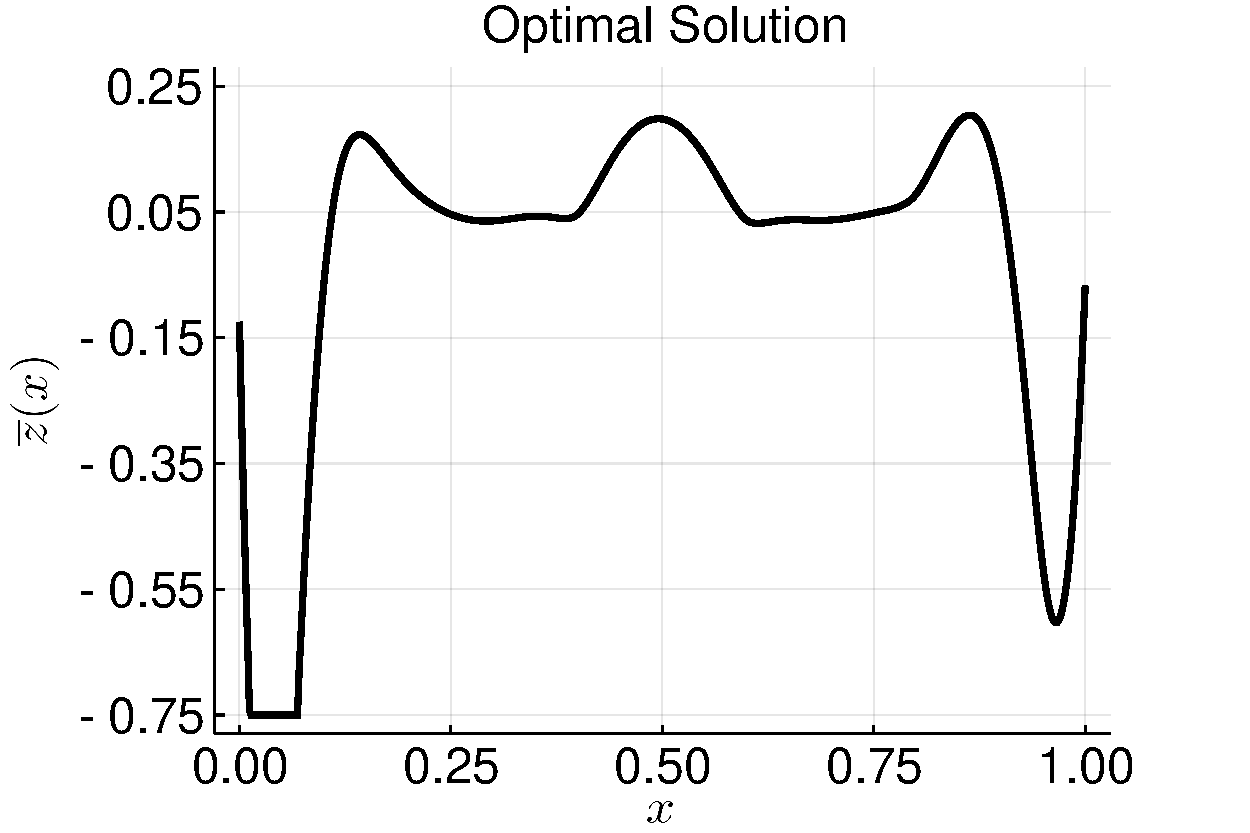
\includegraphics[width=0.47\textwidth]{figures/z_my_1000.pdf}
%  \includegraphics[width=0.47\textwidth]{figures/oos_my_g1000_M2000.pdf}
%%  \caption{(left) Optimal solution $\overline{z}$ up to $\gamma = 1000$. (right) Controlled states using $\overline{z}$ for 2000 out of sample instances of $\bm\xi$. }
%\end{minipage}
%  \caption{\tiny Results of MY, control and oos state. 
%  (left) Total PCG iterations per outer iteration k. (right) Total Newton iterations per outer iteration k.
%  (left) Optimal solution $\overline{z}$ up to $\gamma = 1000$. (right) Controlled states using $\overline{z}$ for 2000 out of sample instances of $\bm\xi$. }
%  \label{fig:my_solutions}
%\end{figure}
%\end{frame}

\begin{frame}\frametitle{Performance Test in 1D: Results and Statistics}
\begin{figure}
     \centering
     \begin{subfigure}[b]{0.25\linewidth}
         \centering
%         \includegraphics[width=\textwidth]{graph1}
         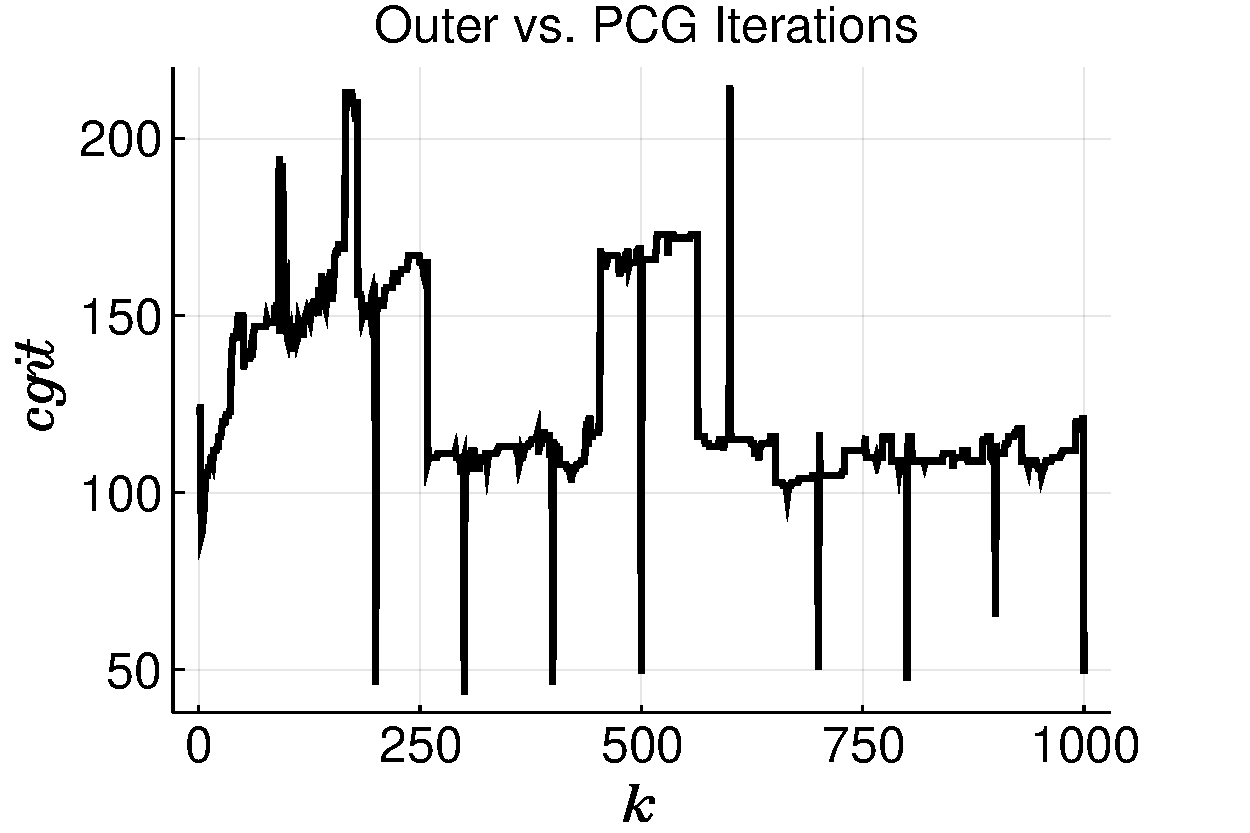
\includegraphics[width=\linewidth]{figures/cg_vec_my_1000.pdf}
         \caption{}
         \label{fig:cq-vs-outer}
     \end{subfigure}\hfill
     \begin{subfigure}[b]{0.25\linewidth}
         \centering
%         \includegraphics[width=\textwidth]{graph2}
         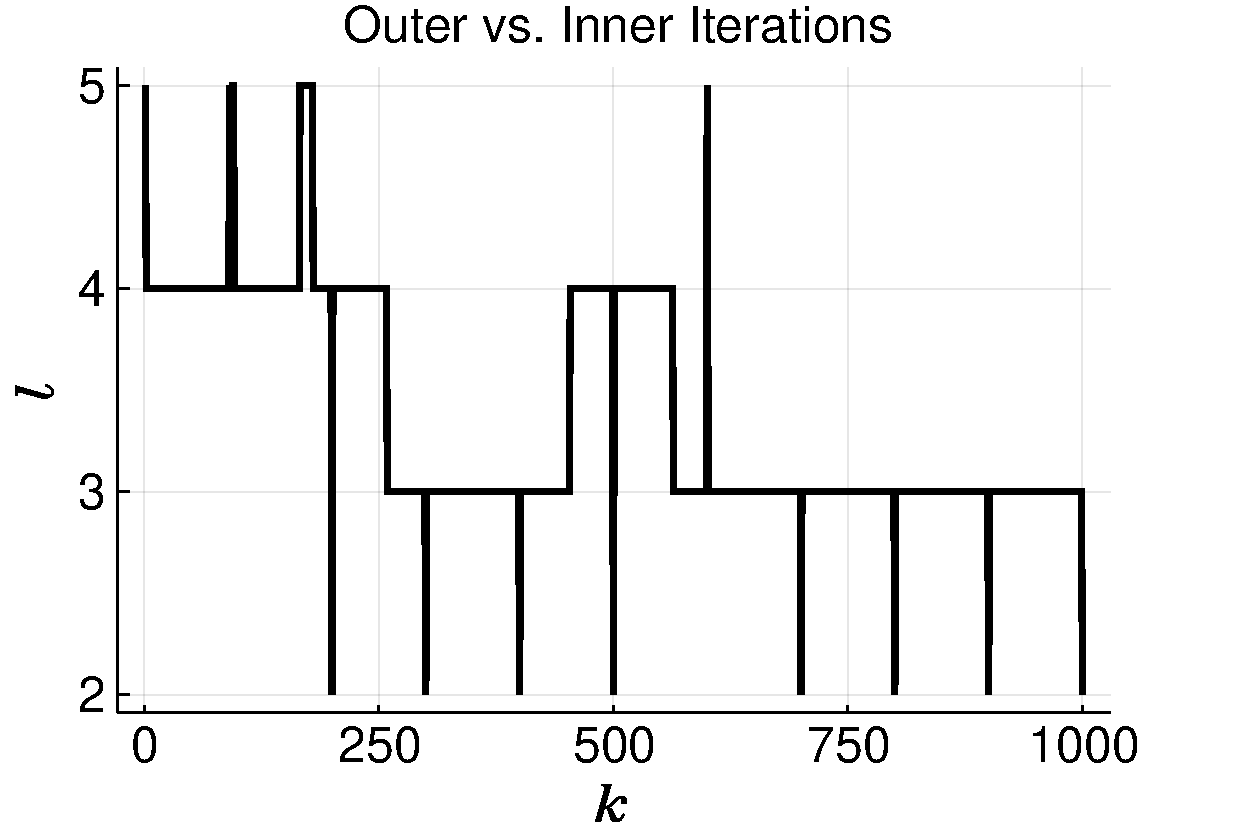
\includegraphics[width=\linewidth]{figures/nwt_vec_my_1000.pdf}
         \caption{}
         \label{fig:nwt-vs-outer}
     \end{subfigure}\hfill
     \begin{subfigure}[b]{0.25\linewidth}
         \centering
%         \includegraphics[width=\textwidth]{graph3}
          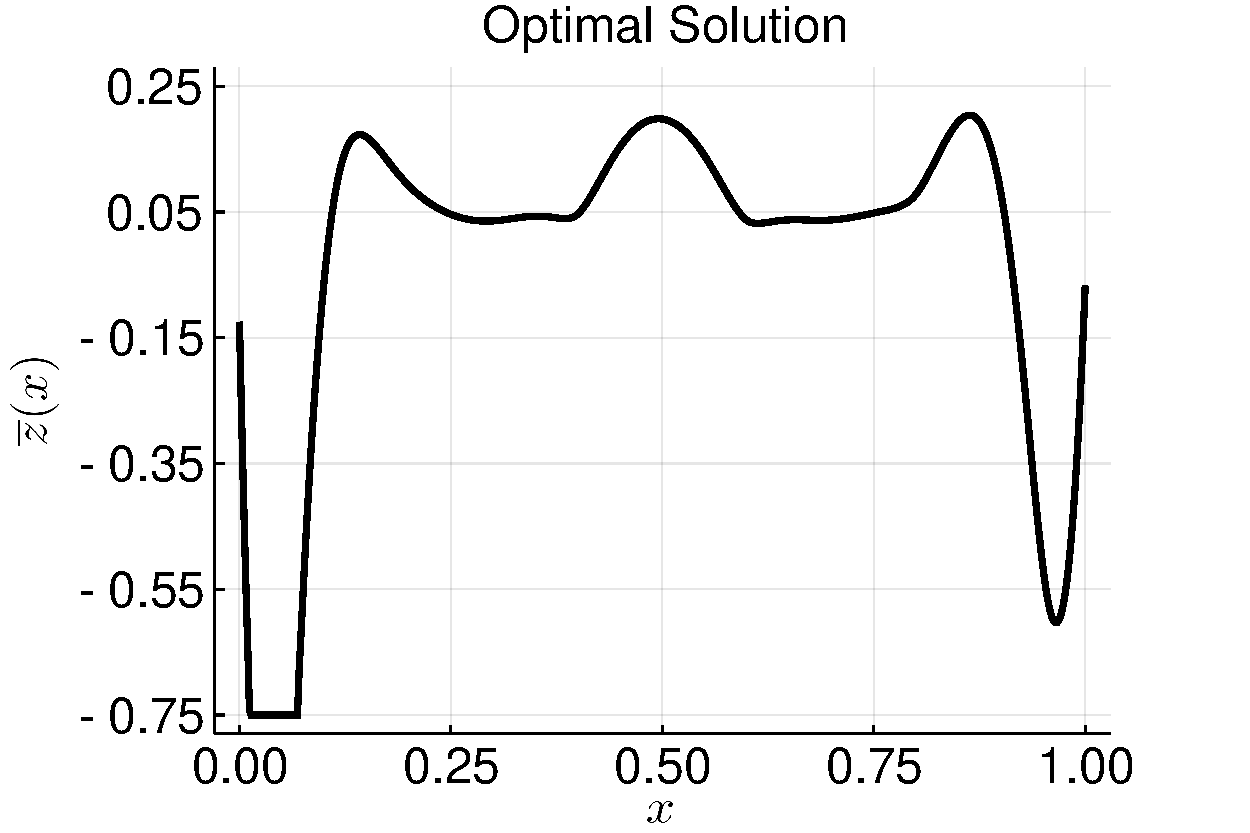
\includegraphics[width=\linewidth]{figures/z_my_1000.pdf}
         \caption{}
         \label{fig:opt-ctrl}
     \end{subfigure}\hfill
     \begin{subfigure}[b]{0.25\linewidth}
     \centering
     \includegraphics[width=\linewidth]{figures/oos_my_g1000_M2000.pdf}
     \caption{}
     \label{fig:oos-states}
 	\end{subfigure}\hfill
        \caption{Performance and computational cost of SAA-semismooth Newton with manual path following.\\
          (a) Total CG iterations until convergence per penalty parameter. \\ (b) Total Newton iterations per penalty parameter. \\
  (c) Optimal solution $\overline{z}$ up to $\gamma = 1000$. \\ (d) Controlled states using $\overline{z}$ for 2000 out of sample instances of $\bm\xi$.\\
 \phantom{A} \\ 
  2.3 \% of cases violate the bound, cf. probability constraints.\\ Algorithm fails if $N$ is too small (10) compared to $\gamma$ (1000).}
        \label{fig:saa-ssn}
\end{figure}
\centering{
Summarizing: SAA $+$ semismooth Newton is robust, but potentially prohibitively expensive.
}
\end{frame}

\begin{frame}[noframenumbering]\thispagestyle{empty}
\vspace*{\fill}
\begin{center}
\Large 
How can we treat the state constraints $\setC$ numerically?\\
\pause
Attempt \# 2: A relaxation approach
\end{center}
\vspace*{\fill}
\end{frame}

\section{Relaxation via Expectation Constraints}
\begin{frame}\frametitle{Functional Reformulation}
\begin{block}{}
\begin{itemize}
\item
Given  $z \in \setZ$ we can define the \textbf{constraint mapping} $\theta(z,\xi)\in H^1(D)$ (pointwise) by
\begin{equation}
\theta(z,\xi)\eqdef \psi(\cdot,\xi)-(u_{f(\cdot,\xi)}+S_{\xi}(z)).
\end{equation}
\item \pause  Observe that $\theta(z,\xibold)\leq 0$ a.s.\
whenever $z\in\setC \cap \setZ_{\rm ad}$ \pause and define 
$\Phi:\setZ\to\R_{+}$ by
\begin{equation}\label{eq:Phi}
\Phi(z)\eqdef\Ex_{\Pr}[F(\theta(z,\xibold))]\qquad\forall z\in\setZ,
\end{equation}
where for measurable functions $v:D\to\mathbb{R}$, $F$ is (\textbf{``average constraint violation in''} $D$) by
\begin{equation}\label{eq:F}
F(v)\eqdef \int_{D}\varphi(v(x))\dif x,
\end{equation}
\item $\varphi : \mathbb R \to \mathbb R_+$ is $C^{1,1}$ convex  and satisfies
$\varphi(r)=0$ for all $r\leq 0$ and
$\varphi(r)> 0$ for all $r>0$.
\end{itemize}
\end{block}\pause
\begin{equation}\label{eq:state_constraint}
\only<4>{S_{\xibold}(z)[x] \geq \psi(x,\xibold)-u_{f(\cdot,\xibold)}(x) \quad \text{for a.a.\ } x\in D \quad\text{a.s.}}
\only<5->{{\color{Red}\Phi(z) \le 0}}
\end{equation}
\end{frame}

\begin{frame}\frametitle{Relaxation and Relation to Probability Constraints}
\begin{block}{}
\begin{itemize}
\item The constraint $\Phi(z) \le \varepsilon$ is not too far from a probability constraint:\pause
\item By Markov's inequality, we
have for any $c > 0$ that
\[
  \Pr( F(\theta(z,\xibold)) \ge c ) \le \frac{1}{c} \Phi(z).
\]
\item \pause
If  $\varepsilon = c^2$, then $z \in \setZ$ such that $\Phi(z) \le \varepsilon$  fulfills %
\[
  \Pr(F(\theta(z,\xibold)) < c) \ge 1 - c.
\]
\item \pause
Probability of infeasibility tamed by choosing moderate
values for $c$; e.g., $c = 10^{-2}$ and $\varepsilon = 10^{-4}$.
\end{itemize}
\end{block}
\end{frame}

\begin{frame}\frametitle{Analysis of $\Phi$}
\centering{
 $\nabla \Phi(z)$ exists and can be calculated using the usual adjoint calculus.
 }
\pause
\begin{theorem}[Kouri, Staudigl, Surowiec (2023)]\label{lem:psi_prop}
  The function $\Phi : \setZ \to \mathbb R_{+}$ is convex,
  globally Lipschitz continuous, and continuously differentiable with
  derivative
  \begin{equation}\label{eq:phi_deriv}
    \Phi'(z) h =\Ex_{\Pr}\left[\left(\varphi'( \theta(z,\xibold)), -S(h)\right)_{L^2(D)}\right]
    \quad\forall\, h\in\scrZ
  \end{equation}
  and Lipschitz continuous gradient,
  \begin{equation}\label{eq:phi_grad}
    \nabla \Phi(z) = -\Ex_{\Pr}[\eta_{\xibold}]
  \end{equation}
  where $\eta=\eta_\xi(z) \in H_0^1(D)$, for fixed $\xi\in\Xi$, fulfills
  \begin{equation}\label{eq:rpde_adj_g}
    \int_{D} \kappa(x,\xi)\nabla \eta(x) \cdot \nabla v(x) \dif x  = \int_{D} \varphi'(\theta(z,\xi))  v(x)  \dif x
      \quad\forall\,v\in H_0^1(D).
  \end{equation}
\end{theorem}

\end{frame}


\begin{frame}\frametitle{Some Useful Bounds for Convergence Analysis}
\centering{
Basic uniform boundedness properties and unbiasedness needed for an oracle can be proven.
}
\pause
\begin{theorem}[Kouri, Staudigl, Surowiec (2023)]\label{prop:stoch-bds}
  Let  Assumptions hold and assume separable differentiable objective $  j(z) = \mathbb E_{\mathbb P}[J_0(u_{\xibold}(z))] + J_1(z)$.
  %\ref{as:j-props}
  \begin{enumerate}
  \item \pause \textbf{Uniformly bounded objective and penalty} There exist constants $M_{\rm obj}$ and $M_{\rm bd}$ such that
%  \begin{equation}\label{eq:simple_bds}
  $
    |j(z)| \le M_{\rm obj} \text{ and }
    |\Phi(z)| \le M_{\rm bd} \quad \forall z \in \setZ_{\rm ad}.
    $
%  \end{equation} 
  \item \pause \textbf{Structured stochastic gradients} The gradient mapping $\nabla_z J(z,\xibold)$ has the form
  \[
    \nabla_z J(z,\xibold) = B^*(\xibold) \lambda_{\xibold} + \nabla J_1(z),
  \]
  where for fixed $\xi\in\Xi$,  $\lambda_{\xi}$ solves
%  \begin{equation}\label{eq:rpde_adj_lam}
  \[
  \int_{D} \kappa(x,\xi)\nabla \lambda(x) \cdot \nabla v(x) \dif x  = -\int_{D} J'_0(u_{\xi}(z))v(x)  \dif x
    \quad\forall\,v\in H_0^1(D).
    \]
%  \end{equation}
  \item \pause \textbf{Bounded stochastic gradients} There exists a constants $M_{\rm adj}$ and  $M_{\rm ctr} > 0$ such that
%  \begin{equation}\label{eq:red_grad_bound}
  $
    \| \nabla_z J(z,\xibold) \|_{\scrZ} \le  M_{\rm adj} \text{ and }
     \| \nabla_z (F \circ \theta)(z,\xibold) \|_{\scrZ} \le  M_{\rm ctr}\quad
    \forall z \in \setZ_{\rm ad},\text{ a.s.}
    $
  \end{enumerate}
\end{theorem}
\end{frame}

\section{An Online Stochastic Approximation Algorithm}
%\begin{frame}\frametitle{}
%\begin{enumerate}
%\item SAA/Empirical approximations + Augmented Lagrangian
%\item OSA
%\item Simple iteration scheme
%\item Iteration scheme with epochs
%\item Theoretical convergence analysis and rates
%\end{enumerate}
%\end{frame}
%
%\begin{frame}[noframenumbering]\thispagestyle{empty}
\begin{frame}\thispagestyle{empty}
\vspace*{\fill}
\begin{center}
\Large 
Can we leverage recent advances in optimization for machine learning and derive a provably convergent algorithm?
\end{center}
\vspace*{\fill}
\end{frame}

\begin{frame}\frametitle{An Online Stochastic Approximation Algorithm (OSA)}
\begin{block}{Motivation}
\begin{itemize}
\item The OSA algorithm is based on work by Yu, Neely, Wei (2017).
\item Their algorithm is inspired by Zinkevich (2003)
\item We extend the Yu, Neely, Wei work to infinite-dimensional Hilbert spaces.
\item We enrich their method by allowing for periodic restarts at pre-defined epochs.
\item This allows for \textbf{larger stepsizes} and appears to be essential in practice.
\end{itemize}
\end{block}

\begin{block}{Related Work}
\begin{itemize}
\item The cooperative stochastic approximation  (CSA) algorithm by G. Lan, Z. Zhou (2020).
\item The conditional gradient method (CndG) by Vladarean, Alacaoglu, Hsieh, Cevher (2020).
\item CSA appears to require an a priori decomposition of the set of iterations.
\item CndG has an iteration complexity of $\scrO(\mathtt{tol}^{-6})$ $\Rightarrow$ $\mathtt{tol} = 10^{-3}$ requires order $10^{18}$ PDE solves.
\end{itemize}
\end{block}
\end{frame}

\begin{frame}\frametitle{OSA Algorithm: Assumptions}
\begin{definition}[Stochastic Oracle]\label{def:so}
Let $(\Omega,\scrF,(\scrF_{k})_{k},\Pr)$ be a filtered probability space. \pause Given
a control $z\in\feas$ and an iteration $k$, a \textbf{stochastic oracle} (SO) outputs a set of \textbf{random elements}
$J_{k}(z)$, $J'_{k}(z)$, $G_{k}(z)$, and $G'_{k}(z)$, with the following properties:\pause
\begin{enumerate}
\item $J_{k}(z)$, $J'_{k}(z)$, $G_{k}(z)$, and $G'_{k}(z)$ are \textbf{unbiased estimators}
of $j(z)$, $\nabla j(z)$, $\Phi(z)-\eps$, and $\nabla \Phi(z)$, respectively, \pause
in the sense that
\begin{equation}\label{eq:unbiased}
\begin{split}
&\Ex[J_{k}(z)\vert\scrF_{k}]=j(z),\quad \Ex[G_{k}(z)\vert \scrF_{k}]=\Phi(z)-\eps,\\
&\Ex[J'_{k}(z)\vert\scrF_{k}]=\nabla j(z),\quad \Ex[G'_{k}(z)\vert \scrF_{k}]=\nabla \Phi(z)
\end{split}
\end{equation}
holds a.s. \pause%\ for all $z\in\feas$.
\item  There exists $D_{1}$ and $D_{2}>0$ independent of $z\in\feas$ and $k\geq 1$:
\begin{equation}\label{eq:gradbound}
\norm{J'_{k}(z)}\leq D_{1}\text{ and } \norm{G'_{k}(z)}\leq D_{2}.
\end{equation} 
\item \pause There exists $M>0$ independent of $z \in \feas$ such that $\abs{G_{k}(z)}\leq M$.
\end{enumerate}
\end{definition}\pause
%\vspace{-2ex}
%\begin{block}{}
\centering{
We proved the necessary bounds for an SO in the PDE-setting.
}
%\end{block}
\end{frame}

\begin{frame}\frametitle{OSA Algorithm: Assumptions}
\begin{block}{}
\begin{itemize}
%\item Proposition 7 provides the necessary bounds for an SO in the PDE-setting.
%\item A common example for an SO is to construct Monte-Carlo estimators
%of the random data involved in the stochastic optimization problem
\item
%\item To obtain
%such an SO, let $m\geq 1$ be a given integer (the sample budget) and assume it
%is easy to simulate $m$ i.i.d.\ copies of the random element $\xibold$. 
Let
$\xi_{k}=(\xi_{k}^{(1)},\ldots,\xi^{(m)}_{k})$ denote a sample of size $m$ at iteration
$k$ and set
\begin{align*}
&J_{k}(z)\eqdef\frac{1}{m}\sum_{t=1}^{m}J(z,{\xi^{(t)}_{k}}),\quad J'_{k}(z)\eqdef\frac{1}{m}\sum_{t=1}^{m}\nabla_z J(z,\xi^{(t)}_{k}),\\
&G_{k}(z)\eqdef\frac{1}{m}\sum_{t=1}^{m}F(\theta(z,\xi^{(t)}_{k})),\quad G'_{k}(z)\eqdef\frac{1}{m}\sum_{t=1}^{m}\nabla_z (F\circ\theta)(z,\xi^{(t)}_{k})
\end{align*}
for all $z\in\feas$. 
%It follows directly from the above discussion that
%this mechanism gives rise to an admissible SO. Note that the generation of
%these estimators requires solving a sequence of PDEs, one for each random
%variable $\xi_{k}^{(t)}$. Hence, the computational complexity of this SO at
%each iteration $k$ is $m\times C$, where $C$ is an upper bound on the cost of
%evaluating the objective function, the constraint, and their derivatives.
\item In the PDE-setting: Need $m$ PDE solves for $J_k$ and $G_k$, $2m$ for $J'_k$ and $G'_k$.
\end{itemize}
\end{block}
\end{frame}

\begin{frame}\frametitle{OSA Algorithm: Basic Form}
\begin{block}{}
\begin{itemize}
\item Given $z\in\feas$ (\textbf{iterate}), $w \ge 0$ (\textbf{weight}), $\gamma > 0$ (\textbf{scaling}), $k \ge 1$ (\textbf{iteration counter}) define:
\begin{equation}\label{eq:functionestimator}
\scrL_{\gamma,k}(z,w)\eqdef J_{k}(z)+\frac{w}{\gamma}G_{k}(z)
\end{equation}
\item This is an estimator of the Lagrangian with multiplier $\mu = w/\gamma$.\pause
\item Query the SO at $(z,w)$ to evaluate $\scrL_{\gamma,k}(z,w)$ and obtain a stochastic gradient
\begin{equation}\label{eq:gradestimator}
\scrL'_{\gamma,k}(z,w)=J'_{k}(z)+\frac{w}{\gamma}G'_{k}(z).
\end{equation}
\item \pause
Given $\alpha > 0$ (\textbf{stepsize}) and $(\con^{1},\pen^{1}) = (z,w)$ generate a sequence $\{(\con^t,\pen^t)\}_{t \in \T}$ by
 \begin{align*}
&\con^{t+1}=P_{\feas}(\con^{t}-\frac{\gamma}{\alpha}\scrL'_{\gamma,t}(\con^{t},\pen^{t})),\\
%\scrP\left(\con^{t},\frac{\gamma}{\alpha}\scrL'_{\gamma,t}(\con^{t},\pen^{t})\right),\\
&\pen^{t+1}=\max\{0,\pen^{t}+G_{t}(\con^{t})+\inner{G'_{t}(\con^{t}),\con^{t+1}-\con^{t}}\},
\end{align*}
where $P_{\feas}(z)\eqdef\argmin_{z'\in\feas}\norm{z'-z}$. 
\end{itemize}
\end{block}
\end{frame}

\begin{frame}\frametitle{OSA Algorithm: Basic Form}
%\begin{algorithm}[t]
\begin{block}{Master Algorithm $\process_{\T}^{(z,w)}(\alpha,\gamma)$}
%\caption{}
\label{alg:master}
\begin{algorithmic}[1]
\STATE{\bfseries Input:} $\T\subseteq\N$ iteration counter set, Initial condition $(z,w)\in\feas\times[0,\infty)$ \;
Parameters $\alpha,\gamma\in(0,\infty)$. 
\STATE{\bfseries Output:} Sequence $\{(\con^{t},\pen^{t}),\min\T\leq t\leq\sup\T+1\}$.
\STATE Set $\con_{\min\T}=z$ and $\pen_{\min\T} = w$\;
\FOR{$t=\min\T,\ldots,\sup\T$}
\STATE Compute $\con^{t+1}=P_{\feas}(\con^{t}-\frac{\gamma}{\alpha}\scrL'_{\gamma,t}(\con^{t},\pen^{t}))$\;
\STATE Compute $\pen^{t+1}=\max\{0,\pen^{t}+G_{t}(\con^{t})+\inner{G'_{t}(\con^{t}),\con^{t+1}-\con^{t}}\}$\;
\ENDFOR
\end{algorithmic}
%\end{algorithm}
\end{block}\pause
\begin{block}{}
\begin{itemize}
\item We can use the Master Algorithm to iterate over ``\textbf{batches}''  $\T_{1},\ldots,\T_{s}$.
\item For each new batch, we have optimization parameters $(\alpha_{j},\gamma_{j}),1\leq j\leq s$. 
\item The initial conditions $(\con_{j}^{1},\pen_{j}^{1}),1\leq j\leq s$, can be chosen using the previous ($j-1$-th) batch.
\item This allows us to build in restarts and longer stepsizes.
\end{itemize}
\end{block}
\end{frame}

\begin{frame}\frametitle{Epoch-based OSA for Larger Stepsizes}
\begin{block}{Epoch-dependent online SA (OSA)}
\label{alg:PDESolve}
\begin{algorithmic}[1]
\STATE{\bfseries Input:} $1\leq\Delta_{N}\leq N$. Initial condition $z_{0}\in\feas$ and $w_{0}=0$\;
Epoch-specific $\{\alpha_{j}\}_{j=1}^{s}$ and $\{\gamma_{j}\}_{j=1}^{s}$\;
\STATE \pause \textbf{Initial values} Set $\con_{0}^{1}=z_0$ and $\pen_{0}^{1} = w_0$\;
\STATE \pause \textbf{Length of batches} Set $s\equiv\lceil\frac{N}{\Delta_{N}}\rceil$\;
\STATE \pause \textbf{Construct} $\T_{0},\T_{1},\ldots,\T_{s}$ with $\T_{0}=\{0\}$, and 
\begin{align*}
\T_{j}&=\{1,\ldots,\Delta_{N}\}\quad\text{ for }1\leq j<s,\quad
\T_{s}=\{1,\ldots,N-(s-1)\Delta_{N}\}. 
\end{align*}
\FOR{$j=1,\ldots,s$}
\STATE \pause \textbf{Initialize with previous steps} Set $\con^{1}_{j}=\con_{j-1}^{\sup\T_{j-1}+1}$ and $\pen^{1}_{j}=\pen_{j-1}^{\sup\T_{j-1}+1}$;
\STATE \pause \textbf{Compute} $\{(\con_{j}^{t},\pen_{j}^{t});1\leq t\leq\sup\T_{j}+1\}$ by calling master algorithm $\process_{\T_{j}}^{(\con_{j}^{1},\pen_{j}^{1})}(\alpha_{j},\gamma_{j})$\;
\ENDFOR
\STATE \pause \textbf{Concatenate trajectories} For $k\in\{1,\ldots,N\}$, set $z_{k}=\con_{j}^{t}$, $w_{k}=\pen_{j}^{t}$ for $k-t=(j-1)\Delta_{N},t\in\T_{j}$\;
\STATE \pause \textbf{Report} $\bar{z}_{N}=\frac{1}{N}\sum_{k=1}^{N}z_{k}.$
\end{algorithmic}
\end{block}
\end{frame}

\begin{frame}\frametitle{Theoretical Convergence Analysis}
\begin{theorem}[Kouri, Staudigl, Surowiec (2023)]\label{prop:feas}
Consider epoch-based OSA algorithm with epochs $j\in\{1,\ldots,s\}$ and
epoch-specific step sizes $\gamma_{j}=\sqrt{\Delta_{N}}$ and
$\alpha_{j}=\Delta_{N}$, where $\Delta_{N}:=\lfloor {\color{Red}N^{a}}\rfloor$ for some ${\color{Red}a\in(0,1]}$. 
Then,
\begin{equation}
\Ex[\Phi(\bar{z}_{N})]\leq \scrO({\color{Red}N^{-a/2}})({\color{Red}1+\scrO(N^{a-1})})+\varepsilon,
\end{equation}
where $\varepsilon>0$ is the a-priori fixed relaxation parameter.
and 
\begin{equation}
\Ex[j(\bar{z}_{N})-j(z^{\star}_{\varepsilon})]\leq\scrO({\color{Red}N^{-a/2}}).
\end{equation}
\end{theorem}
\begin{block}{}
\centering
We sacrifice the theoretical convergence rate derived by Yu, Neely, Wei (2017) ({\color{Red}$a=1$}) for the ability to take \textbf{longer step sizes} and \textbf{restart the algorithm}.
\end{block}
\begin{block}{}
\centering
The numerical experiments, however, indicate that longer step sizes and restarts are essential!
\end{block}
\end{frame}

\section{Numerical Experiments and Hypothesis Testing}


\begin{frame}\frametitle{Example Problem}
%\vspace{-2ex}
\begin{block}{}
%\begin{itemize}
%\item 
We test the OSA algorithm on a strongly convex problem:
\begin{subequations}
  \begin{align}\label{eq:optctrl}
  &\min_{z\in L^2(D)} \; \frac{\alpha}{2}\mathbb{E}\left[\int_D ([u_{\xibold}(z)](x)-w(x))^2\,\mathrm{d}x\right]
                            + \frac{1}{2}\int_D z(x)^2 \,\mathrm{d}x \\
  &\mathrm{subject\;to}\quad -10 \le z \le 10 \quad\text{a.e.}, \qquad u_{\xibold}(z) \ge \psi \quad\text{a.e./a.s.},
  \end{align}
  where $u=u_{\xibold}(z)\in H^1(D)$ is a weak solution to
  \begin{align}\label{eq:pde}
     -\nabla\cdot (\kappa(x,\xi)\nabla u(x)) + v(x,\xi)\cdot\nabla u(x) &= f(x,\xi) + z(x) &&\text{for $x\in D$} \\
     \kappa(x,\xi)\nabla u(x)\cdot n &= 0 && \text{for $x\in\partial D \setminus [\{0\}\times(0,1)]$} \\
     u(x) &= 0 && \text{for $x\in\{0\}\times(0,1)$}
  \end{align}
  for realizations $\xibold = \xi$.
\end{subequations}
Here, $D:=(0,1)^2$, $\alpha=10^4$,\\ $w(x):=(x-0.5)^\top(x-0.5)$, $
  \kappa(x,\xi):= 0.5 + c\exp(\beta(x,\xi)),$  $ 
  v(x,\xi) =  (b(\xi)-a(\xi)x_1, a(\xi)x_2)^{\top},
$\\
%\[
%  \psi(x):= \left\{\begin{array}{cl}
%    \tfrac{1}{4} & \quad\text{if $\|x-(\tfrac{1}{2},\tfrac{1}{2})^\top\|_2\le\tfrac{1}{4}$} \\[2pt]
%    0            & \quad\text{otherwise} \end{array}\right. ,
%\]
$
  \psi(x):= 
    \tfrac{1}{4}, \text{if $\|x-(\tfrac{1}{2},\tfrac{1}{2})^\top\|_2\le\tfrac{1}{4}$ and},
    0,             \text{otherwise};
$\\
%$\Gamma_d: = \{0\}\times(0,1)$, $\Gamma_n:=\partial D\setminus\Gamma_d$,
 $f$ is the sum of five Gaussian sources whose locations, widths and
magnitudes are random. 
%\end{itemize}
\end{block}

\end{frame}

\begin{frame}\frametitle{Computing the Reference Solution}
\vspace{-2ex}
\begin{block}{}
\begin{itemize}
\item For the numerical solution (using SAA) we use continuous P1-FE on a uniform 64×64 quadrilateral mesh.
\item Use SAA with 100 samples and run an augmented Lagrangian-based solver until the optimality and feasibility criteria were smaller than $10^{-8}$.
\item This required 7 \textbf{outer iterations} (12 \textbf{subproblem iterations})
\item The final values for the optimality and feasibility criteria were $5.33 \times 10^{-9}$ and $2.84\times10^{-11}$, respectively. 
\item AL required 20 \textbf{function} and \textbf{gradient evaluations} as well as 145 applications of the \textbf{Hessian} to a vector, resulting in a total of \textbf{495,000 deterministic PDE solves.}
\end{itemize}
\end{block}\pause
\vspace{-2ex}
\begin{block}{}
\begin{itemize}
\item This gives us a \textbf{reference solution} and a \textbf{computational budget.}
\item OSA needs \textbf{3 PDE solves per iteration}. This would amount to $N =$ 165,000 steps.
\item We ran OSA with $N \in \{10^{3}, 10^{4}, 10^{5} \}$ and $\Delta_N = N$ (no restarts), $\Delta_N = 500$.
\item We repeated this five times for each pair of $N$ and $\Delta_N$ to generate statistics.
\end{itemize}
\end{block}
\end{frame}

\begin{frame}[noframenumbering]\thispagestyle{empty}
\vspace*{\fill}
\begin{center}
\Large 
Both SAA and OSA approaches are inherently random.\\ How can we fairly judge the results?
\end{center}
\vspace*{\fill}
\end{frame}

\begin{frame}\frametitle{OSA Experiments: Empirical Distributions}
\begin{figure}[!ht]
\begin{minipage}{0.49\textwidth}
  \centering
  $\Delta_N = N$ \\
  \includegraphics[width=\textwidth]{figures/objective_cdf}\\
%    \includegraphics[width=\textwidth]{objective_cdf}\\
  $J(\overline{z}_N,\xibold)$
\end{minipage}
\begin{minipage}{0.49\textwidth}
  \centering
  $\Delta_N = 500$ \\
  \includegraphics[width=\textwidth]{figures/objective_cdf_delta500}\\
%    \includegraphics[width=\textwidth]{objective_cdf_delta500}\\
  $J(\bar{z}_N,\xibold)$
\end{minipage}
  \caption{\tiny Objective function empirical distribution using $10^4$ samples
           for the SAA optimal
	   control (black) and the OSA controls computed with $10^3$ (red),
           $10^4$ (blue), and $10^5$ (green) iterations for epoch lengths
           $\Delta_N=N$ (left) and $\Delta_N=500$ (right).}
  \label{fig:objective_cdf}
\end{figure}
\end{frame}

\begin{frame}\frametitle{Hypothesis Testing: Kolmogorov-Smirnov}
\begin{block}{}
\begin{itemize}
\item $H_0$ \textbf{null hypothesis}: ``Does the data provide enough evidence to reject this statement?''
\item $H_1$ \textbf{alternative hypothesis}: The negation of $H_0$. \pause
%\item Given $X : (\Omega,\mathcal{F}) \to \mathcal{X}$ r.v. and $R \subset \mathcal{X}$, test if $X \in R$ (reject $H_0$) or $X \not\in R$ (retain $H_0$).
\end{itemize}
\end{block}

\begin{block}{}
\begin{itemize}
\item Given an i.i.d.\ random sample $X_1,\dots,X_n$ and $t \in \mathbb R$, the empirical cdf is defined:
\[
\widehat{F}^{X}_{n}(t)(\omega) := \frac{\# (X_i(\omega) \le t)}{n} = \frac{1}{n} \sum_{i=1}^n I\{X_i(\omega) \le t\}.
\]
\end{itemize}
\end{block}\pause

\begin{block}{Two Sample Kolmogorov-Smirnov}
\begin{itemize}
\item Given two i.i.d r.s. $\{X_i\}_{i=1}^n$, $\{Y_j\}_{j=1}^m$ and their respective cdfs $\widehat{F}^X_{1,n}$, $\widehat{F}^Y_{2,m}$.
\item $H_0$ \textbf{null hypothesis}: 
%Is $\widehat{F}^{X}_{1,n} = \widehat{F}^{Y}_{2,m}$?
%\item
 Are $\{X_i\}_{i=1}^n$ and $\{Y_j\}_{j=1}^m$ drawn from the same distribution?
\end{itemize}
\end{block}
\end{frame}

\begin{frame}\frametitle{Hypothesis Testing: Kolmogorov-Smirnov}
\begin{block}{}
\begin{itemize}
\item We can test $H_0$ by using the KS statistic:
\[
D_{n,m} := \sup_{t \in \mathbb R} |\widehat{F}^{X}_{1,n}(t) - \widehat{F}^{Y}_{2,m}(t)|.
\]
\item Roughly speaking: \textbf{large} $D_{n,m}$ means reject $H_0$, \textbf{small} $D_{n,m}$ means retain $H_0$.\pause
%\item It can be shown that $\mathbb P\left( \sqrt{ \frac{n m}{n + m} } \cdot D \le t \right) \to H(t)$ with $H(t)$ a Jacobi theta function.
%$H(t) = 1 - 2 \sum_{j=1}^{\infty}(-1)^{j-1}\exp(-2j^2 t^2)$. 
\item This yields a ``reject'' relation: \pause
\item Pick $\alpha \in (0,1)$ ($100 \times \alpha =$  the probability of rejecting $H_0$ given when it is actually true).
\item \pause Compute $D_{n,m}$
\item \pause If
\[
    D_{n,m} > \sqrt{-\ln\left(\frac{\alpha}{2}\right)\cdot\frac{n+m}{2nm}},
\]
then $D_{n,m}$ too large.
%\item Type I error: $\alpha \in (0,1)$ ($100 \times \alpha =$  the probability of rejecting $H_0$ given when it is actually true).
%\item Typically $\alpha$ is chosen between $0.2$ and $0.001$.
%The type I error rate is the probability of rejecting the null hypothesis given that it is true. The test is designed to keep the type I error rate below a prespecified bound called the significance level, usually denoted by the Greek letter α (alpha) and is also called the alpha level. Usually, the significance level is set to 0.05 (5%), implying that it is acceptable to have a 5% probability of incorrectly rejecting the true null hypothesis.[7]

\end{itemize}
\end{block}

\end{frame}

\begin{frame}\frametitle{KS-Test for the OSA Algorithm}
\begin{block}{}
\begin{itemize}
\item Given a numerically computed ``optimal'' control $z$, we define two types of random variables
\[
\aligned
J(z,\xibold) &: \text{(possible objective function values at the solution $z$)}\\
F(\theta(z,\xibold)) &: \text{(possible penalty function values at the solution $z$)}\\
\endaligned
\]
\item For two controls $z_1$ and $z_2$ we ask: 
\[
\aligned
&\text{$H_0$ \textbf{objective}: $\widehat{F}^{J(z_1)}_m \stackrel{?}{=}  \widehat{F}^{J(z_2)}_m$}\quad \text{$H_0$ \textbf{penalty}:  $\widehat{F}^{F(\theta(z_1))}_m \stackrel{?}{=}  \widehat{F}^{F(\theta(z_2))}_m$}\\
\endaligned
\]
\item We use sample size $m = 10^4$ and generate \textit{new} realizations, which leads to samples
$\{ J(z_i,\xibold_1), \dots, J(z_i,\xibold_m)\}$
$\{ F(\theta(z_i,\xibold_1)), \dots, F(\theta(z_i,\xibold_m))\}$ for $i = 1,2,...$
\end{itemize}
\end{block}
\end{frame}

\begin{frame}\frametitle{KS Test Summary}
\begin{block}{}
\begin{itemize}
\item We {\color{Blue}retain} $H_0$ \textbf{objective} when comparing OSA controls for $\alpha \le 0.17$:
\begin{center}
\textit{
OSA controls computed using the same $N$ and $\Delta_N$ generate values of $J(z,\xi)$ that are drawn from the same distribution.
}
\end{center}\pause
\item We {\color{Red}reject} $H_0$ \textbf{objective} when comparing SAA and OSA controls:
\begin{center}
\textit{
SAA and OSA controls using the same $N$ (and $\Delta_N = N$ or $500$) generate values of $J(z,\xi)$ that are not drawn from the same distribution.
}
\item The probability of a type I error (rejecting $H_0$ when it is true) is close to zero, i.e. $\alpha \le 10^{-20}$:
\end{center}%\pause
%\item For $N = 10^5$ and $\Delta_N = 500$ it appears that the SAA and OSA controls generate \textit{penalty function values} drawn from the same distribution.
\end{itemize}
\end{block}\pause
\begin{block}{}
\centering We can get ``close'' to the performance of an algorithm that uses second order information with OSA and roughly the same budget, but the statistics indicate we need more effort to get closer.
\end{block}
\end{frame}

\section{Conclusion \& Outlook}
\begin{frame}\frametitle{}
\begin{block}{}
\begin{enumerate}
\item State constraints in OUU present a major theoretical and numerical challenge.
\item Previous approaches require a lot of structure or CQs/penalty approaches.
\item Using a degenerate functional reformulation of the constraint, we arrive at a numerically tractable relaxation that has ties to probability constraints.
\item We presented an epoch-based online SA algorithm that can perform well compared to a second-order algorithm using SAA with judiciously chosen restart parameters. 
\item Hypothesis testing should become a part of our numerical experiments in OUU!
\item Missing results: ``Full convergence'' theory for FEM (mesh refinement) + OSA (sampling): FEM adds bias to estimators $J_k, J'_k$ etc.
\item More missing results: Asymptotic statistics for SAA (Monte Carlo) approximation to justify second-order algorithms.
%\item Preprint available upon request!
\end{enumerate}
\end{block}\pause
\centering
{\Huge Thank You!}\\
\url{https://github.com/thomas-surowiec/cmai-talk-2024-ol}
\end{frame}

\end{footnotesize}
\end{document}